\documentclass[spanish,a4paper,12pt,oneside,notitlepage]{extreport}

%%%%%%%%%%%%%%%%%%%%%%%%%%%%%%%%%%%%%%%%%%%%%%%%%%%%%%%%%%%%%%%%%%%%%%%%%%%%%%%
\usepackage{graphicx}
\usepackage{epsfig}
\usepackage[utf8]{inputenc}
\usepackage[spanish]{babel}
\usepackage{alltt}
\usepackage{algorithm}
\usepackage{algorithmic}
\usepackage{multirow}
\usepackage[top=3cm, bottom=3cm, left=3cm, right=3cm]{geometry}
\usepackage{libertinus}
\usepackage[T1]{fontenc}
\usepackage{titlesec}
\usepackage{csquotes}
% \usepackage[ttdefault=true]{AnonymousPro}
\usepackage[font=small,labelfont=bf]{caption}
\usepackage{setspace}
\usepackage[labelfont=bf]{subcaption}
\usepackage[dvipsnames]{xcolor}
\usepackage{url}
\usepackage{listings}
\usepackage{hyperref}
\usepackage{wrapfig}
\usepackage{lipsum}
\usepackage{tabularx}
\usepackage{rotating}


\usepackage{courier}
\lstset{basicstyle=\footnotesize\ttfamily,breaklines=true}

\usepackage[style=numeric,sorting=none]{biblatex}
\addbibresource{report.bib}
 
\setcounter{secnumdepth}{3}
\setcounter{tocdepth}{3}
 
\captionsetup{font={small,stretch=0.95}}
 
\newcommand{\SONY}{{\sc Sony}}
\newcommand{\MICROSOFT}{{\sc Microsoft}}
\newcommand{\GCC}{\textsf{\textsc{G}CC}}
\newcommand{\INTEL}{\textsf{\textsc{I}ntel}}

%%% Traducimos el pseudocodigo
\renewcommand{\algorithmicwhile}{\textbf{mientras}}
\renewcommand{\algorithmicend}{\textbf{fin}}
\renewcommand{\algorithmicdo}{\textbf{hacer}}
\renewcommand{\algorithmicif}{\textbf{si}}
\renewcommand{\algorithmicthen}{\textbf{entonces}}
\renewcommand{\algorithmicrepeat}{\textbf{repetir}}
\renewcommand{\algorithmicuntil}{\textbf{hasta que}}
\renewcommand{\algorithmicelse}{\textbf{en otro caso}}
\renewcommand{\algorithmicfor}{\textbf{para}}

%\newcommand{\RETURN}{\textbf{retornar} }
\newcommand{\RET}{\STATE \textbf{retornar} }
\newcommand{\TO}{\textbf{hasta} }
\newcommand{\AND}{\textbf{y} }
\newcommand{\OR}{\textbf{o} }

\renewcommand{\baselinestretch}{1.1} 


%%%%%%%%%%%%%%%%% Creamos un entorno para listar código fuente %%%%%%%%%%%%%%%
\newenvironment{sourcecode}
{\begin{list}{}{\setlength{\leftmargin}{1em}}\item\scriptsize\bfseries}
{\end{list}}

\newenvironment{littlesourcecode}
{\begin{list}{}{\setlength{\leftmargin}{1em}}\item\tiny\bfseries}
{\end{list}}

\newenvironment{summary}
{\par\noindent\begin{center}\textbf{Abstract}\end{center}\begin{itshape}\par\noindent}
{\end{itshape}}

\newenvironment{keywords}
{\begin{list}{}{\setlength{\leftmargin}{1em}}\item[\hskip\labelsep \bfseries Keywords:]}
{\end{list}}

\newenvironment{palabrasClave}
{\begin{list}{}{\setlength{\leftmargin}{1em}}\item[\hskip\labelsep \bfseries Palabras clave:]}
{\end{list}}


%%%%%%%%%%%%%%%%%%%%%%%%%%%%%%%%%%%%%%%%%%%%%%%%%%%%%%%%%%%%%%%%%%%%%%%%%%%%%%%
% Format
%%%%%%%%%%%%%%%%%%%%%%%%%%%%%%%%%%%%%%%%%%%%%%%%%%%%%%%%%%%%%%%%%%%%%%%%%%%%%%%
%\usepackage{showframe}
%\marginparwidth 0mm
%%\topmargin -4 mm
%\topmargin -21 mm
%\headheight 10 mm
%\headsep 10 mm

%\textheight 229 mm
%\textheight 246 mm

%\oddsidemargin -5.4 mm
%\evensidemargin -5.4 mm
%\oddsidemargin 5 mm
%\evensidemargin 5 mm

%\oddsidemargin -3 mm
%\evensidemargin -3 mm

%\textwidth 17 cm
%\textwidth 15 cm
%\columnsep 10 mm

\input{amssym.def}

%%%%%%%%%%%%%%%%%%%%%%%%%%%%%%%%%%%%%%%%%%%%%%%%%%%%%%%%%%%%%%%%%%%%%%%%%%%%%%%

\begin{document}

%%%%%%%%%%%%%%%%%%%%%%%%%%%%%%%%%%%%%%%%%%%%%%%%%%%%%%%%%%%%%%%%%%%%%%%%%%%%%%%
% First Page
%%%%%%%%%%%%%%%%%%%%%%%%%%%%%%%%%%%%%%%%%%%%%%%%%%%%%%%%%%%%%%%%%%%%%%%%%%%%%%%

\pagestyle{empty}
\thispagestyle{empty}

\newcommand{\HRule}{\rule{\linewidth}{1mm}}
\setlength{\parindent}{0mm}
\setlength{\parskip}{0mm}


\vspace*{\stretch{0.3}}
\begin{center}
  % \includegraphics[scale=0.8]{images/logo_vertical}\\[10mm]
  
\includegraphics[scale=1]{images/logo-esit}\\[10mm]
  \vspace*{\stretch{0.5}}
  {\huge \scshape Trabajo de Fin de Grado}
\end{center}

\HRule
\begin{center}
  \vspace{1em}
  {\Huge Planificación optimizada de un sistema de semáforos mediante algoritmos evolutivos: una aplicación a la rotonda del Padre Anchieta, en Santa Cruz de Tenerife} \\[3mm]
  \rule{5cm}{0.6pt}\\[5mm]
  {\Large \textit{Optimized planning of a traffic light system using evolutionary algorithms: an application to the Padre Anchieta roundabout, in Santa Cruz de Tenerife}} \\[3mm]
  \rule{5cm}{0.6pt}\\[5mm]
  {\Large Francisco Arturo Cruz Zelante}
\end{center}
\HRule

\vspace*{\stretch{2}}

\begin{center}
  \Large San Cristóbal de La Laguna, \today
\end{center}

\titleformat{\chapter}[display]
{\normalfont%
    \LARGE% %change this size to your needs for the first line
    \itshape}{\chaptertitlename\ \thechapter}{20pt}{%
    \normalfont \bfseries \Huge %change this size to your needs for the second line
}


%%%%%%%%%%%%%%%%%%%%%%%%%%%%%%%%%%%%%%%%%%%%%%%%%%%%%%%%%%%%%%%%%%%%%%%%%%%%%%%
\newpage{\pagestyle{empty}}
\thispagestyle{empty}
%%%%%%%%%%%%%%%%%%%%%%%%%%%%%%%%%%%%%%%%%%%%%%%%%%%%%%%%%%%%%%%%%%%%%%%%%%%%%%%

% \pagestyle{myheadings} %my head defined by markboth or markright
% % No funciona bien \markboth sin "twoside" en \documentclass, pero al
% % ponerlo se dan un montón de errores de underfull \vbox, con lo que no se
% % ha puesto.
% \markboth{Francisco Arturo Cruz Zelante}{Planificación optimizada de un sistema de semáforos mediante algoritmos evolutivos: una aplicación a la rotonda del Padre Anchieta, en Santa Cruz de Tenerife}

%Numeracion en romanos
\renewcommand{\thepage}{\roman{page}}
\setcounter{page}{1}

\newpage{\pagestyle{empty}}
\thispagestyle{empty}

\chapter*{}
\begin{flushright}
    {\Huge\textbf{Agradecimientos}}
    \bigskip
    \bigskip

    {\itshape
        A vosotros, Eduardo y Gara, por tutorizarme\\
        durante este proyecto y por vuestra inestimable \\
        ayuda para sacarlo adelante,
        \bigskip
        
        A ti, Edu, por confiar en mí y ofrecerme \\
        la beca de colaboración,
        \bigskip
        
        A vosotros, papá y mamá, por el cariño \\ 
        incondicional y el soporte durante la carrera,
        \bigskip
        
        A vosotros, mis compañeros, por ayudarme a lo largo de \\
        la carrera y estar siempre dispuestos a echarme un cable, \\
        ya fuera para un algoritmo o para una cerveza,
        \bigskip

        A la vieja guardia, por estar ahí,
        \bigskip
        
        Y a todas las personas que, de algún modo u otro, \\
        me han llevado al lugar donde estoy hoy.
        \bigskip
        
        }
\end{flushright}


\newpage{\pagestyle{empty}}
\thispagestyle{empty}
\pagestyle{empty}

\begin{center}
    \textbf{Resumen}
\end{center}

La rotonda del Padre Anchieta (Tenerife) está situada en una posición estratégica al conectar el corazón académico, de ocio, comercial y urbanístico de la ciudad de La Laguna; por lo que asume una cantidad sustancial de tráfico que, en horas punta, suele causar atascos importantes. Con el objetivo de aliviar la congestión del tráfico, este proyecto estudia la instalación de semáforos en la rotonda, optimizando la duración de las fases de estos gracias a un algoritmo evolutivo. Para ello se emplea Genetics.js, una librería programada en TypeScript orientada a algoritmos evolutivos; y SUMO, un simulador de tráfico microscópico de código abierto.

\medskip

La simulación se realiza gracias a dos archivos básicos: el archivo de red, que no es más que un mapa de la rotonda de Padre Anchieta obtenido de OpenStretMap y convertido al formato del empleado por SUMO; y el archivo de tráfico, generado gracias a una herramienta del simulador, \texttt{flowrouter.py}, que genera rutas de tráfico a partir de datos de aforadores. Estos datos fueron provistos por el Cabildo de Tenerife, en un estudio realizado en la rotonda por la corporación en 2019. 

\medskip

Se han evaluado siete casos distintos respecto a la rotonda, tres de ellos sin semáforos y los otros cuatro con semáforos; modificando la cantidad de peatones y las configuraciones semafóricas en cada uno de ellos. Para determinar qué parámetros del algoritmo evolutivo proporcionaban los mejores resultados, se llevó a cabo un estudio estadístico previo en función de dos parámetros: el tipo de cruce y el tamaño de la población. Finalmente, una vez realizado el estudio estadístico previo y la simulación de cada caso, se concluyó que el empleo de semáforos optimizados no consigue mejorar el tráfico de la rotonda; y que el incremento de los peatones ralentiza de modo perceptible el tráfico rodado. Una serie de mejoras propuestas como trabajo futuro se incluye al final de esta memoria.

\medskip

\noindent \textbf{Palabras clave:} SUMO, simulación, tráfico, algoritmos evolutivos, TypeScript, semáforos, planificación, optimización

\newpage
\pagestyle{empty}

\bigskip
\bigskip

\begin{center}
    \textbf{Abstract}
\end{center}

The Padre Anchieta roundabout (Tenerife) is located in a strategic position by connecting the academic, leisure, commercial and urban heart of the city of La Laguna; so it takes on a substantial amount of traffic which, at peak times, often causes major traffic jams. With the aim of alleviating traffic congestion, this project studies the installation of traffic lights in the roundabout, optimizing the duration of the phases of these thanks to an evolutionary algorithm. For this, Genetics.js is used, a TypeScript library oriented to evolutionary algorithms; and SUMO, an open source microscopic traffic simulator.

\medskip

The simulation is carried out thanks to two basic files: the network file, which is nothing more than a map of the Padre Anchieta roundabout obtained from OpenStretMap and converted to the format used by SUMO; and the traffic file, generated thanks to a simulator tool, \texttt{flowrouter.py}, which generates traffic routes based on gauge data. These data were provided by the Tenerife Island Council, in a study carried out by the corporation in the roundabout in 2019.

\medskip

Seven different cases have been evaluated with respect to the roundabout, three of them without traffic lights and the other four with traffic lights; modifying the number of pedestrians and the traffic light configurations in each of them, when applicable. To determine which parameters of the evolutionary algorithm provided the best results, a previous statistical study was carried out based on two parameters: the type of crossing and the size of the population. Finally, once the previous statistical study and the simulation of each case had been carried out, it was concluded that the use of optimized traffic lights did not improve traffic in the roundabout; and that the increase in pedestrians noticeably slows down road traffic. A series of improvements proposed as future work is included at the end of this report.

\medskip

\noindent \textbf{Keywords:} SUMO, traffic, simulation, evolutionary algorithms, TypeScript, traffic lights, scheduling, optimization



\tableofcontents

\newpage{\pagestyle{empty}}
\listoffigures

\newpage{\pagestyle{empty}}
\listoftables

\newpage{\pagestyle{empty}}

% \setlength{\parindent}{6mm}
\setlength{\parskip}{4mm}

%Numeracion a partir del capitulo I
\renewcommand{\thepage}{\arabic{page}}
\setcounter{page}{1}
\pagestyle{plain}

\chapter{Introducción}
\label{cap:intro}

La rotonda de Padre Anchieta (cuyo nombre oficial es «glorieta del Brasil») toma su nombre por la escultura en representación del beato José de Anchieta, colocada en el centro de la rotonda, y regalada por el pueblo brasileño en 1960~\cite{gallo_glorieta_2013}.

\begin{figure}[H]
    \centering
    \includegraphics[width=\textwidth]{report/images/padre-anchieta.png}
    \caption[Mapeado en 3D de la Rotonda del Padre Anchieta.]{Mapeado en 3D de la Rotonda del Padre Anchieta. Cortesía de Google Earth\protect\footnotemark}
    \label{fig:padre_anchieta_3d}
\end{figure}

\footnotetext{Véase \url{https://earth.google.com/web/@28.48023943,-16.31770104,534.93762391a,251.9187181d,35y,-46.25428648h,74.81244137t,0r}}

La popularidad de la rotonda se explica por su posición estratégica, rodeada de viviendas, comercios, dos campus universitarios de la Universidad de La Laguna (Central y Anchieta), y por la cual pasa una de las principales autopistas de la isla, la TF-5; además de conectar otras cuatro vías: la Carretera de la Esperanza (TF-24), la Carretera de Geneto (TF-263), la Avenida de la Trinidad y la Avenida Astrofísico Francisco Sánchez. Sin embargo, los orígenes de la rotonda son considerablemente más humildes (véase la Figura~\ref{fig:anchieta_ev}).

Hoy en día, y después de varias obras, la rotonda ha incrementado considerablemente su tamaño y el tráfico que circula a través de ella, especialmente en horas punta. Es normal que en dichas horas se produzcan retenciones muy importantes y, en determinadas situaciones, un bloqueo total del tráfico; a veces durante horas (véase~\cite{gulesserian_vuelven_2018}, a modo de ejemplo). Las grandes cantidades de tráfico que absorbe la rotonda, y los bloqueos y ralentizaciones que se producen como consecuencia, tienden a afectar al tráfico de la TF-5, causando retenciones a la altura de la rotonda.

La optimización del tráfico en la rotonda se convierte, por tanto, en un asunto de primer orden respecto de la movilidad en la isla. La rotonda da una vía a los estudiantes tanto del norte como del sur que van a clase, a los trabajadores que se dirigen hacia La Laguna y hacia Santa Cruz; y en general a una gran cantidad de trayectos entre ambas ciudades y el norte de la isla que no puede dejarse desatendida.

\begin{figure}[h]
    \centering
    \begin{subfigure}[t]{.49\textwidth}
      \centering
      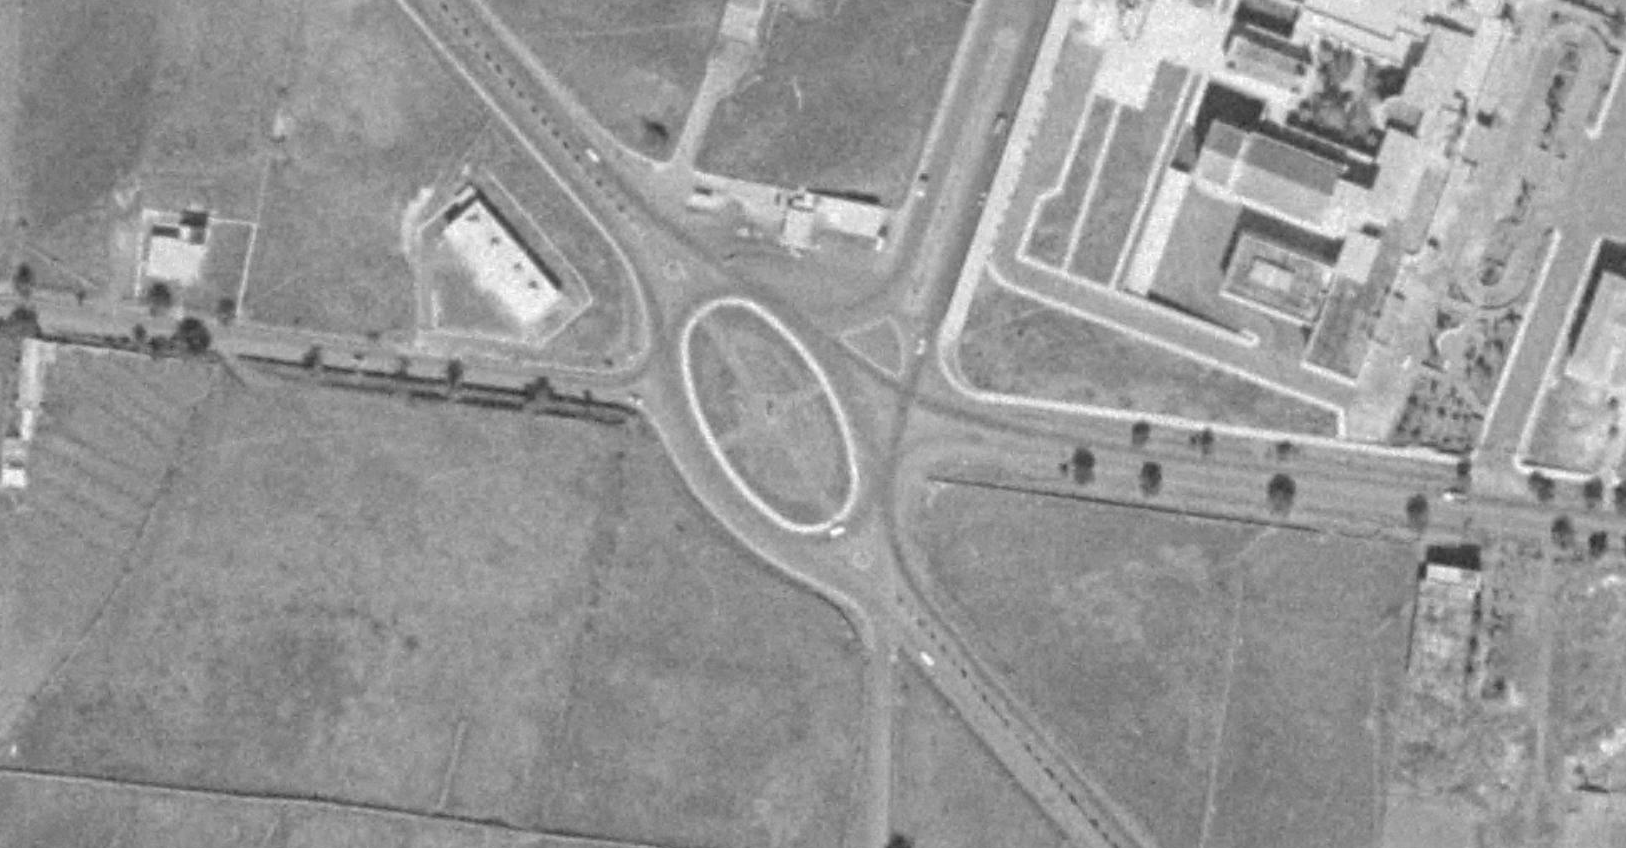
\includegraphics[width=\textwidth]{report/images/amp-anchieta-1964.png}
      \caption{1964}
      \label{fig:anchieta1964}
    \end{subfigure}
    \hfill
    \begin{subfigure}[t]{.49\textwidth}
      \centering
      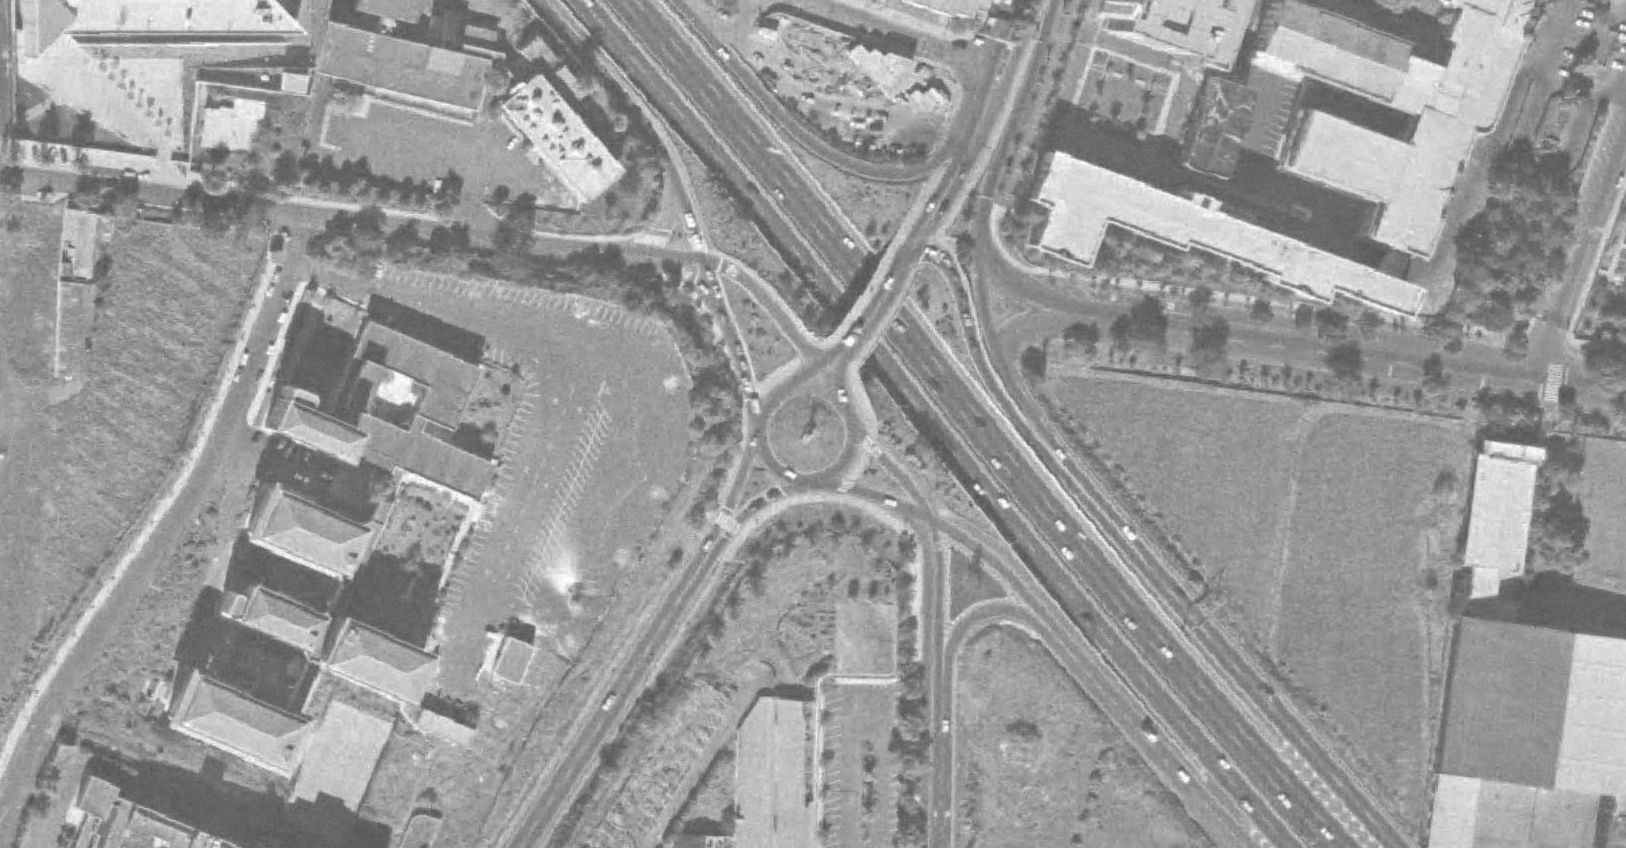
\includegraphics[width=\textwidth]{report/images/amp-anchieta-1994.png}
      \caption{1994}
      \label{fig:anchieta1994}
    \end{subfigure}
    \vspace{0.7cm}
    \begin{subfigure}[t]{.49\textwidth}
      \centering
      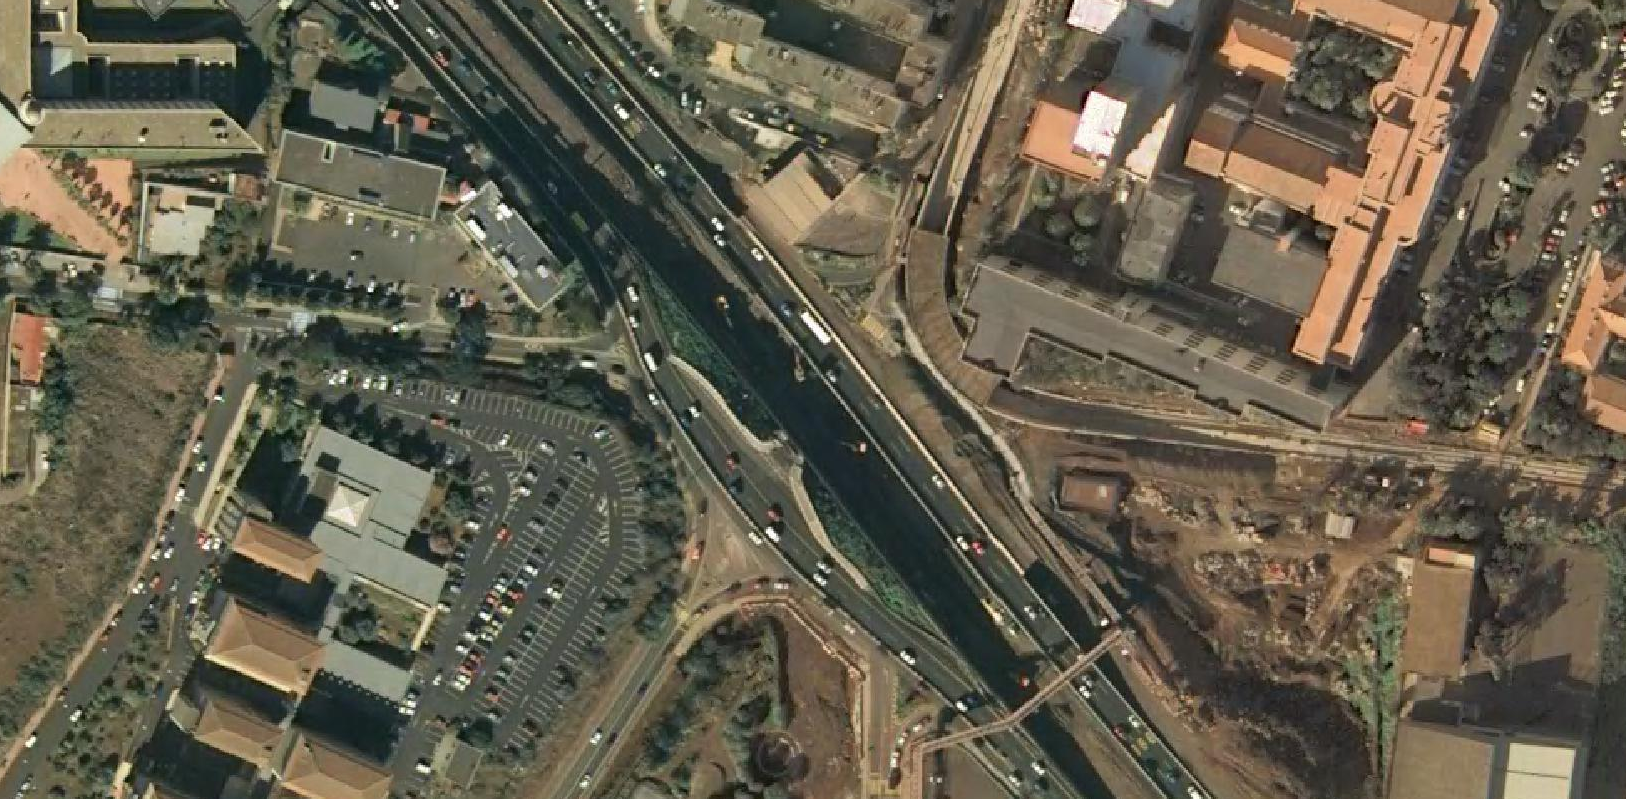
\includegraphics[width=\textwidth]{report/images/amp-anchieta-2006.png}
      \caption{2006 (en obras)}
      \label{fig:anchieta2006}
    \end{subfigure}
    \hfill
    \begin{subfigure}[t]{.49\textwidth}
      \centering
      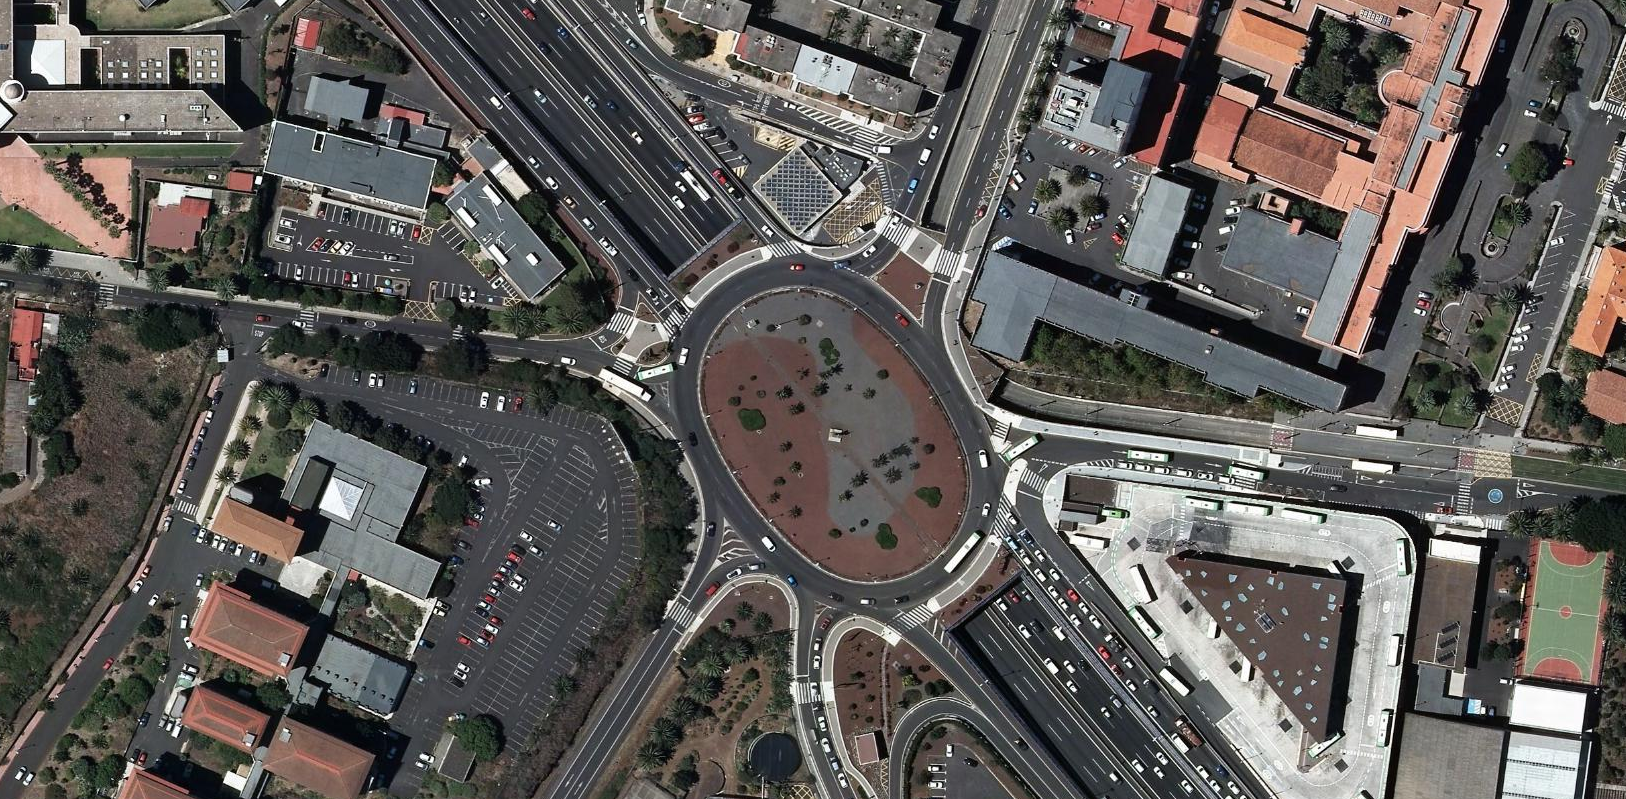
\includegraphics[width=\textwidth]{report/images/amp-anchieta-2019.png}
      \caption{2019}
      \label{fig:anchieta2019}
    \end{subfigure}
    \caption[Evolución de la rotonda de Padre Anchieta a lo largo de los años.]{Evolución de la rotonda de Padre Anchieta a lo largo de los años. Fotografías cortesía de GRAFCAN\protect\footnotemark}
    \label{fig:anchieta_ev}
\end{figure}

\footnotetext{Véase \url{https://visor.grafcan.es/visorweb/}}

Las autoridades de la isla no son ajenas al problema de tráfico que plantea la rotonda. El Cabildo de Tenerife, organismo de cuya competencia depende la rotonda, y el Gobierno de Canarias, de cuya competencia depende la TF-5, han planteado varias medidas, de entre las cuales cabe mencionar:

\begin{itemize}
    \item El soterramiento de la TF-24 en dirección hacia Santa Cruz (a la espera de ejecutar el proyecto)~\cite{dia_cabildo_2019}.
    \item La construcción de una pasarela de peatones sobre la rotonda~\cite{rozas_pasarela_2019}.
    \item La potenciación del vehículo compartido y el transporte público: creación de carriles BUS-VAO en la TF-5~\cite{20minutos_gobierno_2019}.
    \item Las propuestas para la construcción de nuevas líneas de tranvía~\cite{redaccion_de_eldiarioes_cabildo_2020}.
\end{itemize}

Sin embargo, todas las medidas mencionadas suponen un cargo importante al erario público, suponen una carga administrativa importante (por todos los procesos de licitación y control que han de realizarse), llevan mucho tiempo construirlas y mientras dure el proceso resultarán un incordio para los conductores y usuarios de la vía.


\section{Objetivos}

Con la elaboración de este proyecto lo que se propone es la instalación de semáforos en la rotonda, cuyas duraciones de fase se optimicen mediante un algoritmo evolutivo. De esta forma, se podrá comprobar si con la instalación de estos semáforos es posible mejorar la circulación del tráfico en función de determinados parámetros como: la duración media de los trayectos de los vehículos, la velocidad media de los vehículos, la cantidad de vehículos que han logrado completar su trayecto en
un tiempo determinado, etc.
% Gara
%una hora, etc.

El problema que se pretende abordar no es otro que el de la planificación de la duración de las fases de los semáforos, más conocido como el \textit{Traffic Light Scheduling Problem} (TLSP). Este problema de optimización plantea cuánto deberían durar las fases de los semáforos de uno o varios cruces para mejorar la circulación con respecto a varios parámetros; el más habitual de ellos siendo el tiempo medio de viaje de un grupo de vehículos desde un origen hasta el destino. Otros parámetros, como la distancia media o la contaminación de los vehículos también pueden ser tenidos en cuenta a la hora de evaluar el comportamiento de las distintas configuraciones semafóricas.

En comparación con las medidas antes mencionadas, la que se propone en este trabajo supone un coste considerablemente más bajo, no molestaría tanto a los conductores durante la instalación (la cual sería también mucho más corta y sencilla) y plantea una solución muy interesante que podría ser reaprovechada para otras vías sin coste alguno (si ya tuvieran semáforos instalados).

Para llevar a cabo el proyecto, se han empleado principalmente las dos herramientas siguientes:

\begin{itemize}
    \item La primera de ellas es \textit{SUMO}~\cite{lopez_microscopic_2018}, un simulador de tráfico microscópico que nos permitirá evaluar cómo se comporta el tráfico en la rotonda de Padre Anchieta, con datos de tráfico provistos por el Cabildo de Tenerife.
    \item La segunda es \textit{Genetics.js}~\cite{abrante_dorta_framework_2019}, una librería orientada a algoritmos evolutivos (en particular, algoritmos genéticos) programada en \textit{TypeScript}.
\end{itemize}


\section{Optimización mediante algoritmos evolutivos}

Los algoritmos evolutivos toman como guía la evolución biológica y la llevan al campo de la optimización. A diferencia de otros métodos, esta clase de algoritmos busca ofrecer mejores resultados mediante la evolución de los individuos de una población, haciéndolos mutar, combinando características entre ellos y seleccionando los mejores candidatos a optar a solución de un problema~\cite{eiben_introduction_2003} (normalmente, de optimización no lineal con un amplio espacio de búsqueda), donde otros algoritmos tardarían demasiado o serían directamente inviables.

Este tipo de algoritmos se componen de varios elementos~\cite{eiben_introduction_2003}:

\begin{itemize}
    \item \textbf{Representación.} Es la manera en que representamos los individuos. Para el caso que aquí nos atañe, un individuo es una intersección vial con un conjunto de semáforos. La duración de cada una de las fases de esos semáforos, así como los retardos, se representan como un vector de números. Cada individuo es una posible solución.
    \item \textbf{Función de evaluación (fitness).} Devuelve un valor, a partir de un individuo, que determina qué tan bueno es como solución al problema.
    \item \textbf{Población}. Conjunto de individuos. Es útil para determinar cuantos individuos vamos a forzar a competir entre sí en una generación.
    \item \textbf{Mecanismo de selección de padres.} Se corresponde con los criterios tenidos en cuenta a la hora de determinar cuáles queremos que sean los individuos que se reproducirán en la generación, normalmente de carácter estocástico.
    \item \textbf{Operadores (recombinación y mutación).} Determinan la manera en que se alteran los individuos de la población.
    \item \textbf{Mecanismo de selección de supervivientes (reemplazo).} Se centra en seleccionar a los individuos que formarán parte de la siguiente generación de entre la población padre y la población hija a partir de los operadores genéticos. Este mecanismo, a diferencia del de selección de padres, suele ser un método determinista basado en el fitness.
    \item \textbf{Inicialización y terminación.} Finalmente, debemos determinar de qué manera queremos iniciar el algoritmo (normalmente, con individuos generados aleatoriamente) y cómo queremos terminarlo (por ejemplo, tras un número determinado de iteraciones, o en función de un umbral, tomando como guía el \textit{fitness} o la diversidad entre individuos).
\end{itemize}


% Gara:
% Yo creo que empezaría la frase diciendo algo como "este tipo de algoritmos se utilizarán para optimizar los tiempos y fases del conjunto de semáforos
Este tipo de parámetros se pueden emplear en la función de evaluación del algoritmo evolutivo para calcular el valor que correspondería a un individuo; en este caso, un conjunto de semáforos. En el capítulo~\ref{cap:simulacion} se detallarán los parámetros tenidos en cuenta en dicha función, así como otros aspectos relevantes relacionados con el planteamiento del problema.

Así pues, el TLSP busca solventar los tiempos que han de asignarse a cada fase de un conjunto de semáforos, buscando que tales tiempos se ajusten a determinadas restricciones y que sean óptimos. Una fase de un conjunto de semáforos es un momento determinado en que cada semáforo alumbra un color distinto. Por ejemplo: tomando en cuenta dos semáforos $S_1$ y $S_2$, una fase en concreto se correspondería con el semáforo $S_1$ en rojo y el semáforo $S_2$ en ámbar.

Cuando tratamos con varios conjuntos de semáforos es normal que algunas ciudades planteen una sincronización entre estos a través de retardos, denominadas <<oleadas de verde>>, lo que en determinadas circunstancias optimiza la circulación de vehículos. Este retardo también se ha tenido en cuenta en la evaluación del algoritmo.

Para obtener estos valores es necesario simular el comportamiento de los vehículos con las distintas configuraciones de semáforos. Para esto se ha empleado SUMO, un simulador de tráfico microscópico de código abierto, que nos proveerá con los argumentos necesarios para la función de evaluación.

La obtención de los datos necesarios para realizar las simulaciones, como el mapa de la localización que queremos simular, así como los datos de circulación de los vehículos, han sido obtenidos: de un lado, de \textit{OpenStreetMap} (para el caso del mapa); y de otro, del Cabildo de Tenerife (para el caso de los datos de circulación de la zona en cuestión). De esto se hablará con extensión en los siguientes capítulos, pues el tratamiento de estos datos conforma una parte importante del proyecto. La Figura~\ref{fig:evolutionary_alg_graph} sintetiza el proceso de trabajo principal del proyecto descrito en estos párrafos.
% Gara: creo que primero pondría la gráfica y luego empezaría a explicar a partir de ella, indicando el capítulo/s en el que se desarrolla cada paso...

\begin{figure}[!t]
    \centering
    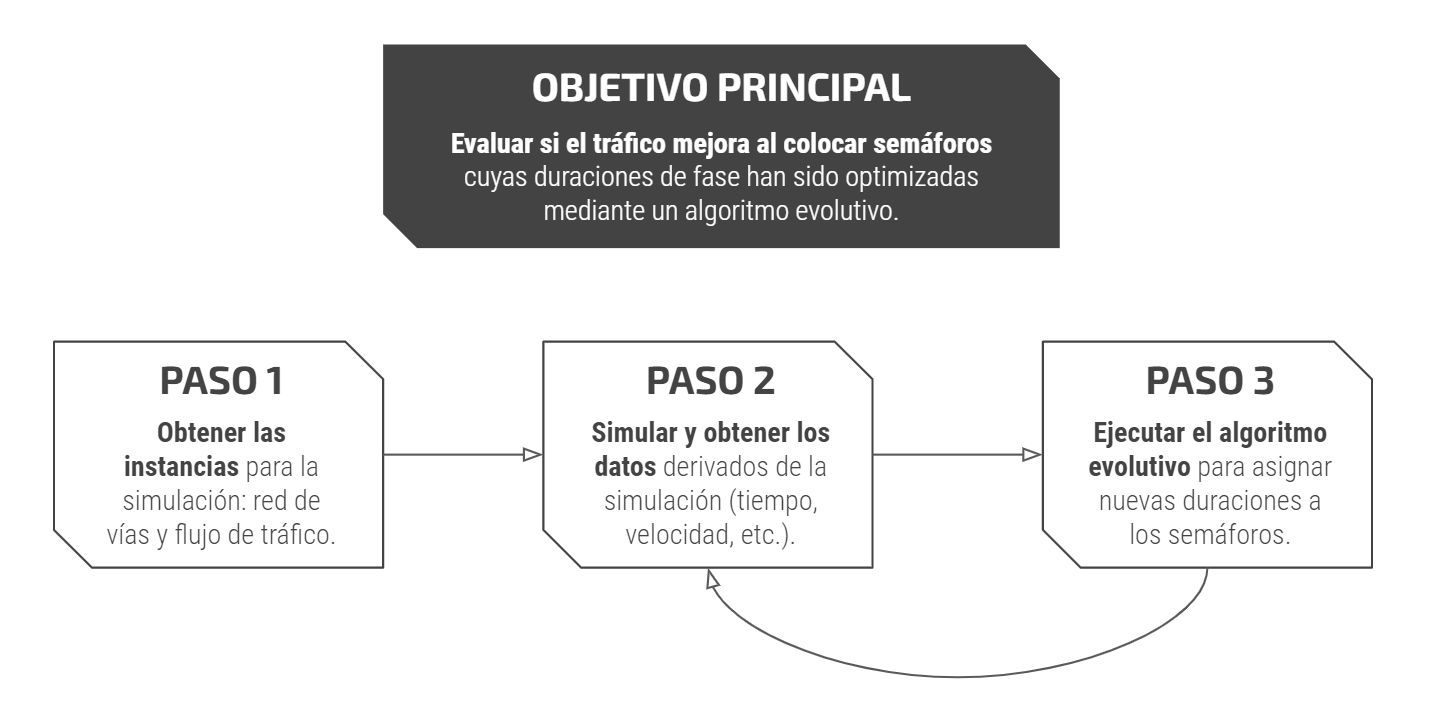
\includegraphics[width=\textwidth]{report/images/evolutionary_alg_graph.png}
    \caption{Gráfica del proceso general del trabajo.}
    \label{fig:evolutionary_alg_graph}
\end{figure}

La zona seleccionada para llevar a cabo la simulación ha sido la de la glorieta del Brasil (más conocida como la rotonda del Padre Anchieta), sita en San Cristóbal de La Laguna. La elección de esta zona en particular viene determinada por la gran cantidad de tráfico que absorbe cada día, al estar situada en el corazón del municipio, al haber una gran variedad de viviendas, comercios y lugares de trabajo en las zonas conexas, así como por la presencia de dos campus universitarios pertenecientes a la Universidad de La Laguna. La rotonda no tiene semáforos, por lo cual en este proyecto se han planteado varias configuraciones semafóricas.

Por tanto, lo que se plantea en este proyecto es la obtención de una instancia real, con datos de tráfico incluidos, de la rotonda del Padre Anchieta. Los resultados de la simulación del tráfico realizada por SUMO en dicha instancia servirán de entrada a un algoritmo evolutivo para evaluar si, incluyendo semáforos en la rotonda y optimizando la duración de las fases, es posible mejorar la circulación en función de los parámetros especificados.


\section{Trabajos previos relacionados}

El planteamiento aquí propuesto ya ha sido tratado desde distintas perspectivas por otros autores en los que se basa este trabajo, de entre los que cabe resaltar los siguientes:

\begin{itemize}
    \item Segredo \textit{et al.}~\cite{segredo_optimising_2019}. El artículo versa sobre el TLSP y el empleo de varios optimizadores mono y multi-objetivos basados en la diversidad, por ser mucho más eficientes y, en consecuencia, ser capaces de lidiar con zonas significativamente más grandes de ciudades como Berlín, París, Estocolmo o Málaga, llegando a simular casi 1000 intersecciones y más de 2600 vehículos.
    \item Sánchez \textit{et al.}~\cite{sanchez_applying_2008}. El artículo, de 2008, versa también sobre el TLSP pero aplicado a las Ramblas, en Santa Cruz de Tenerife. El autor, con la optimización propuesta de las duraciones de las fases de los semáforos, consigue mejoras notables en la circulación del tráfico.
    \item Dorta Acosta~\cite{dorta_acosta_simulacion_2019}. En este caso se trata de un TFG de un compañero de la Escuela Superior de Ingeniería y Tecnología, que versa sobre la instalación de semáforos inteligentes en la rotonda de Padre Anchieta.
\end{itemize}


\chapter{Definición de las instancias: archivo de red y tráfico}
\label{cap:instancias}

\section{Definición de la zona de simulación: el archivo de red}
\label{def_zona_sim_archivo_red}

\subsection{Generación y conversión}
\label{gen_conv}

La zona de la rotonda del Padre Anchieta ha sido extraída de \textit{OpenStreetMap} (OSM), servicio gracias al cual ha sido posible obtener una representación fiel y bastante completa de la rotonda y las vías conexas. OSM permite seleccionar una zona del mapa y descargarla en formato \texttt{.osm}.

Aunque inicialmente se había seleccionado una zona considerable grande de la rotonda (incluyendo, por ejemplo, calles de la zona de la Av. Trinidad, como la Obispo Rey Redondo; así como vías de la zona del Coromoto), finalmente se seleccionó una zona que únicamente abarca la rotonda, las entradas y salidas y el tramo de la TF-5 que pasa por debajo, incluyendo las entradas y salidas de la autopista. Esto se debe a que los datos de tráfico disponibles se circunscriben únicamente a las zonas mencionadas, por lo que no se podría haber simulado otras vías conexas sin perder fiabilidad en la simulación (al tener que aproximar los datos de los vehículos que circulan por dichas vías, en vez de contar con datos empíricos).

OSM ofrece los datos en formato <<.osm>>; sin embargo, los archivos de red legibles por SUMO y las demás herramientas del simulador siguen un formato XML con extensión \texttt{.net.xml}. Para realizar la conversión se empleó una de las herramientas que viene con el simulador, denominada \texttt{NETCONVERT}. Esta herramienta está específicamente destinada a importar archivos redes viales de diferentes fuentes para generar redes viales que puedan ser utilizadas por otras herramientas~\cite{noauthor_netconvert_nodate} (como SUMO, NetEdit, etc.).

% El comando empleado para ejecutar \texttt{NETCONVERT} fue el siguiente:

% \begin{lstlisting}[breaklines=true]
% netconvert --type-files osmNetconvert.typ.xml,osmNetconvertPedestrians.typ.xml --osm-files <Archivo OSM> --output-file <Nombre del archivo de salida> --geometry.remove --roundabouts.guess --ramps.guess --junctions.join --tls.guess-signals --tls.discard-simple --tls.join --no-turnarounds.except-deadend --crossings.guess --osm.all-attributes --sidewalks.guess
% \end{lstlisting}

Los archivos \texttt{xml} que se pasan al comando vienen predefinidos en el pack de herramientas de SUMO, y sirven principalmente para definir el modo en que se clasificarán las vías en el momento de convertirlas (por ejemplo, qué vías se clasificarán como calles o autopistas, con qué velocidad, etc.), así como la adición de aceras y pasos peatonales. El resto de \textit{flags} señalan a \texttt{NETCONVERT} cómo debe realizar la conversión (por ejemplo, pidiendo que infiera las intersecciones, los carriles de aceleración y desaceleración de las autopistas, etc.).

El archivo que obtenemos como resultado del proceso de conversión es con el cual podemos empezar a trabajar con SUMO y las herramientas que trae consigo.

\subsection{Limpieza}

\subsubsection{Intersecciones}

Pese a que \texttt{NETCONVERT} hace un excelente trabajo generando el archivo de red, todavía es necesario realizar pequeños cambios antes de que pueda llevarse a cabo la simulación. Esto se realizó mediante \texttt{NETEDIT}, otra de las herramientas que viene en el paquete de SUMO, y que está orientada a editar archivos de red mediante una GUI, ya sea para modificar las vías (o los metadatos de estas), la forma de las intersecciones, los semáforos, el orden de preferencias en las vías, y toda una serie de funcionalidades relacionadas~\cite{noauthor_netedit_nodate}. El trabajo principal que se ha realizado en este aspecto tiene que ver con la forma de las intersecciones. 

La manera en que dos vías se conectan en SUMO (y, por extensión, en \texttt{NETEDIT}) viene determinada por el Modelo de Intersección de Vías de SUMO~\cite{erdmann_sumos_2014}. Explicado superficialmente, en SUMO la red de vías se representa mediante un grafo. Una intersección consiste en un nodo \textit{de entrada} y otro \textit{de salida} (donde un nodo representa una vía con un identificador concreto, y que sea de entrada o de salida implica de dónde viene y hacia donde va un vehículo). Así pues, un carril de entrada puede tener varios carriles de salida posibles (o sea, varios destinos que puede tomar un vehículo en una intersección).

Bien, dentro de esta intersección existen los denominados <<carriles internos>>, que conectan los nodos de entrada con los de salida y permiten especificar con exactitud por donde deben circular los vehículos en la intersección. Estos carriles internos son calculados automáticamente por \texttt{NETCONVERT}, pero a veces falla o los calcula de una manera inexacta, lo que provoca que algunas intersecciones proporcionadas por el conversor no representen con fidelidad la  intersección real.

Asimismo, es muy importante configurar bien las intersecciones puesto que son necesarias para añadir los semáforos y configurarlos adecuadamente en función de las vías que vaya a regular; situación que también se da para los pasos de peatones.

La mayoría del trabajo de limpieza consistió, pues, en procurar la exactitud de las intersecciones de las vías de entrada y salida de la rotonda. Esto es posible modificando la forma de estas en \texttt{NETEDIT}; pero, por desgracia, es un trabajo en gran parte tedioso y a veces frustrante, puesto que la manera en que están definidas estas intersecciones es mediante un conjunto de puntos (que encierran la zona por la que pasan los carriles internos, como se ve en la figura~\ref{fig:interseccion3}). 

\begin{figure}[ht]
    \centering
    \begin{subfigure}[t]{.30\textwidth}
      \centering
      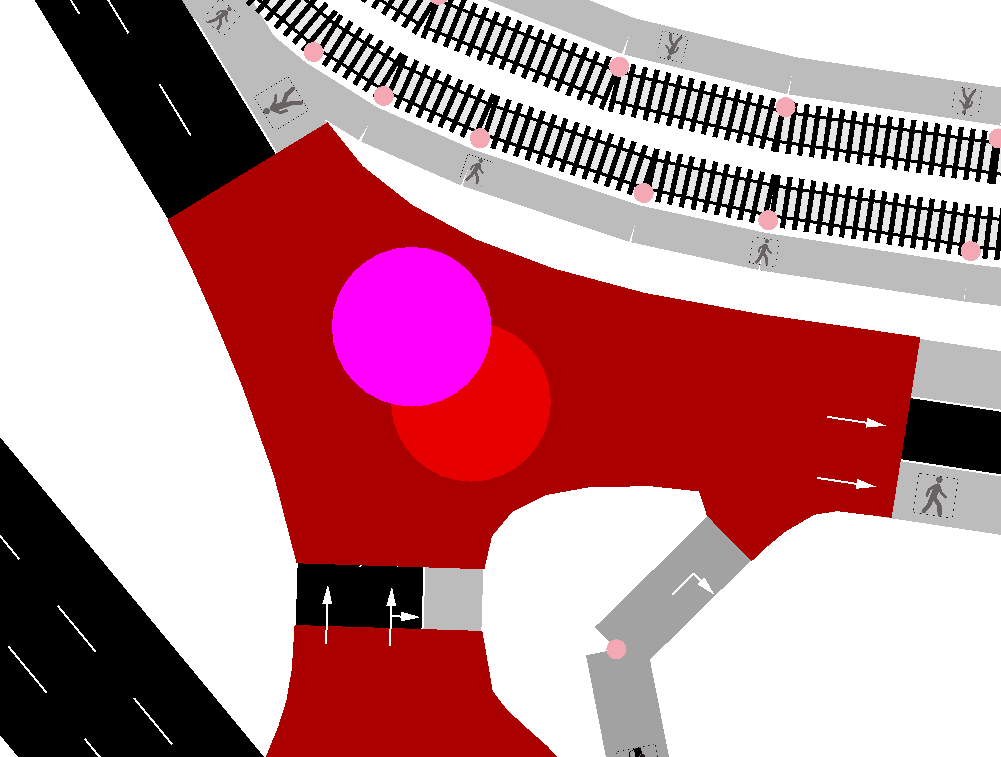
\includegraphics[width=\textwidth]{report/images/interseccion1.png}
      \caption{Forma de la intersección (señalada en rojo).}
      \label{fig:interseccion1}
    \end{subfigure}
    \hfill
    \begin{subfigure}[t]{.30\textwidth}
      \centering
      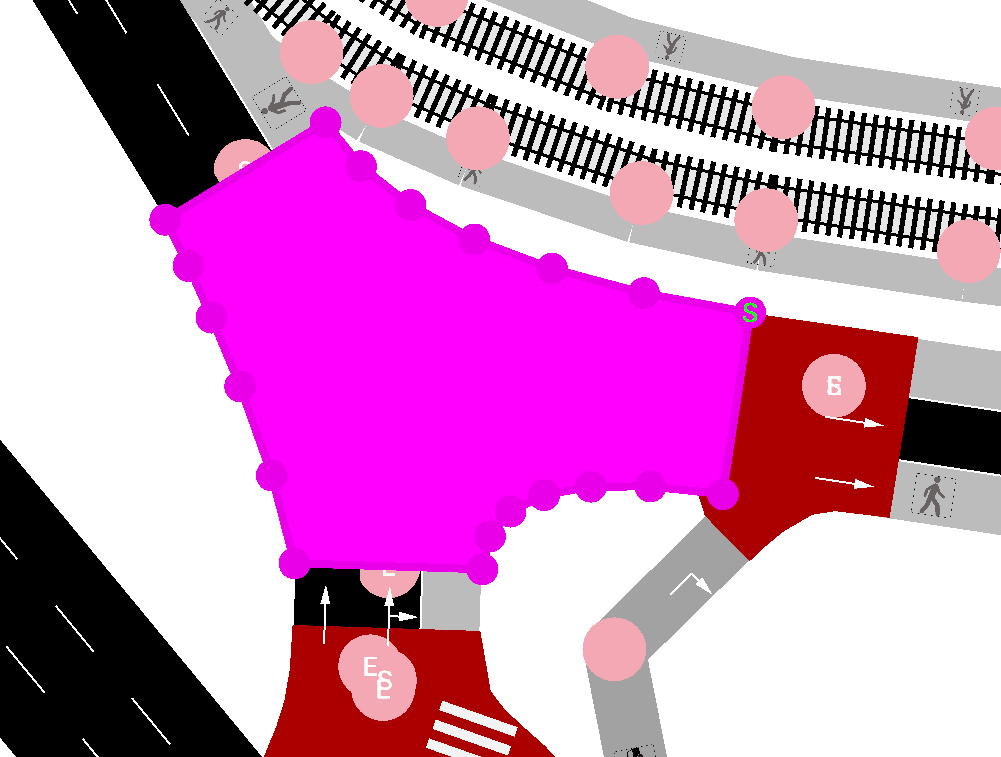
\includegraphics[width=\textwidth]{report/images/interseccion2.png}
      \caption{Modo de edición de la intersección (en violeta). Se aprecian los puntos que definen la forma.}
      \label{fig:interseccion2}
    \end{subfigure}%
    \hfill
    \begin{subfigure}[t]{.30\textwidth}
      \centering
      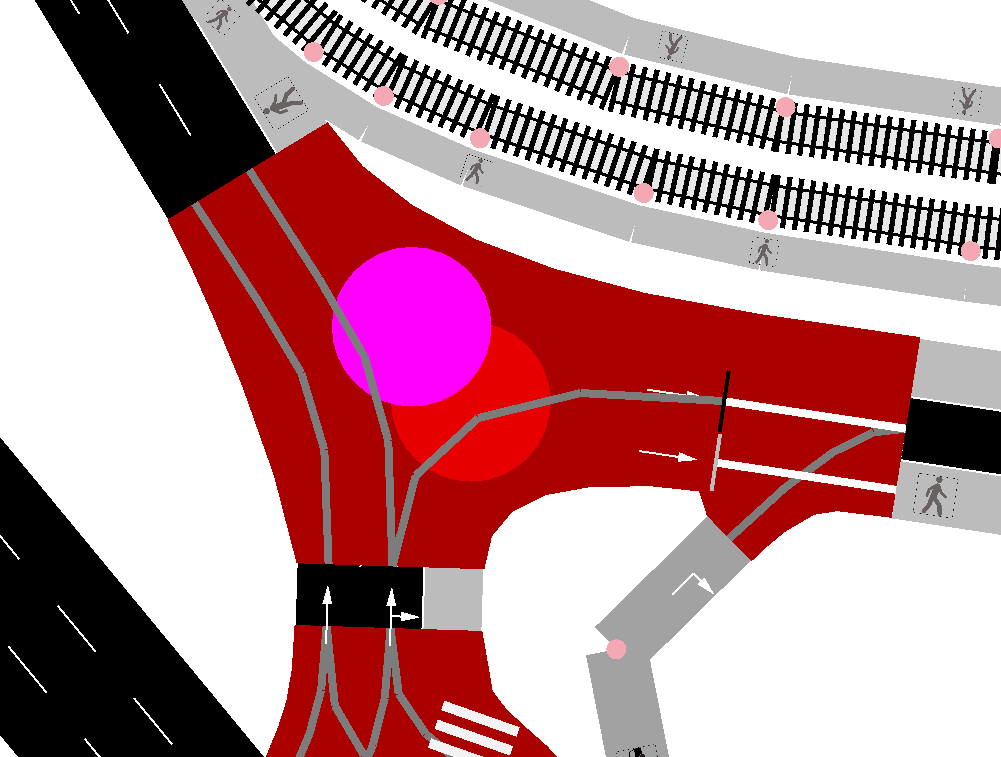
\includegraphics[width=\textwidth]{report/images/interseccion3.png}
      \caption{Carriles internos (señalados en gris). La forma de estos depende de la forma de la intersección.}
      \label{fig:interseccion3}
    \end{subfigure}
    \caption{Representación de las intersecciones en \texttt{NETEDIT}.}
    \label{fig:interseccion}
\end{figure}

Además, cabe mencionar que \texttt{NETEDIT}, en determinadas circunstancias o al intentar algunas modificaciones en concreto, ha llegado a cerrarse de forma inesperada debido a un error interno del programa, resultando además que se perdía todo el trabajo realizado hasta el momento, por lo que había que empezar de nuevo.

\subsubsection{Vías mal priorizadas}

Para señalar la prioridad de una vía sobre otra, SUMO asigna un \textit{valor de prioridad} en función del tipo de vía que sea, de acuerdo con una clasificación que también emplea \textit{OpenStreetMap}. Por ejemplo, una autopista tiene prioridad sobre las carreteras primarias, estas sobre las carreteras secundarias, estas sobre las calles urbanas, etc. 

Durante el proceso de conversión es posible que algunas vías no estén señaladas o priorizadas adecuadamente, dando lugar a que los ceda el paso se produzcan por vías a las que en realidad les corresponde la prioridad en una intersección. Este fue el caso de algunas entradas de la rotonda.

Hay una \textit{flag} que se puede añadir al comando \texttt{NETCONVERT} mencionado en la sección~\ref{gen_conv} que se denomina \texttt{--roundabouts.guess}. Esta \textit{flag} permite que, durante el proceso de conversión, se detecten automáticamente las rotondas y se ajusten las prioridades de acuerdo con la norma general: las vías de la rotonda en sí tienen prioridad sobre las vías de entrada. Sin embargo, al ser un método heurístico, es posible que falle y es el caso ante el cual nos encontramos.

Por suerte, corregirlo no es particularmente complicado. Basta con reducir el valor de prioridad de la vía de entrada con respecto al de la rotonda y problema solucionado.

\subsubsection{Vías mal representadas}

Este es un caso bastante particular y tiene que ver con la salida de la TF-5, en dirección norte, que permite incorporarse a la rotonda de Padre Anchieta (representado en la figura \ref{fig:salida-tf5-norte}). 

\begin{figure}[ht]
    \centering
    \begin{subfigure}[t]{0.48\textwidth}
      \centering
      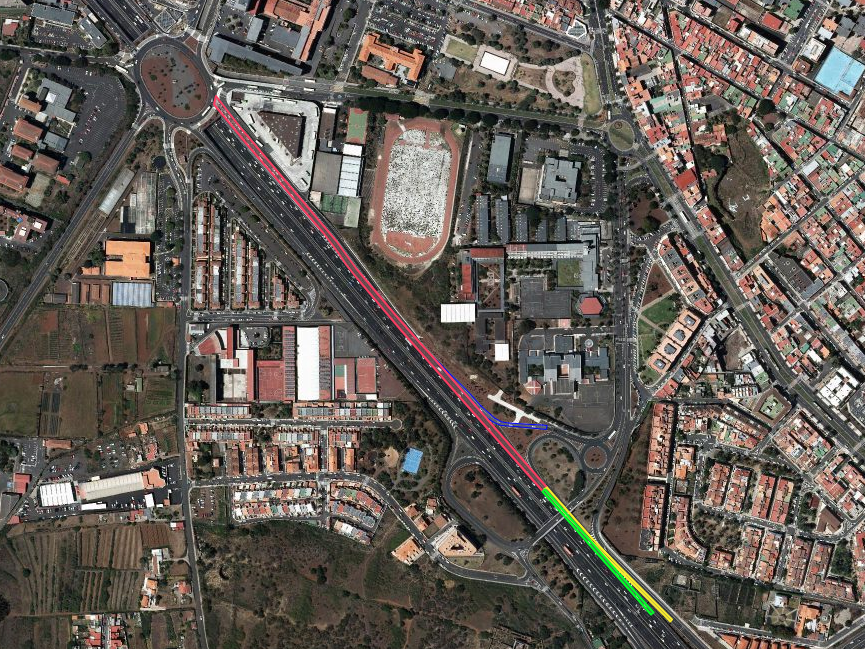
\includegraphics[width=\textwidth]{report/images/salida-tf5-norte-lejos_.png}
      \caption{La salida de la TF-5 (dir. norte) a la rotonda de Padre Anchieta vista desde lejos.}
      \label{fig:salida-tf5-norte-lejos}
    \end{subfigure}
    \hfill
    \begin{subfigure}[t]{0.48\textwidth}
      \centering
      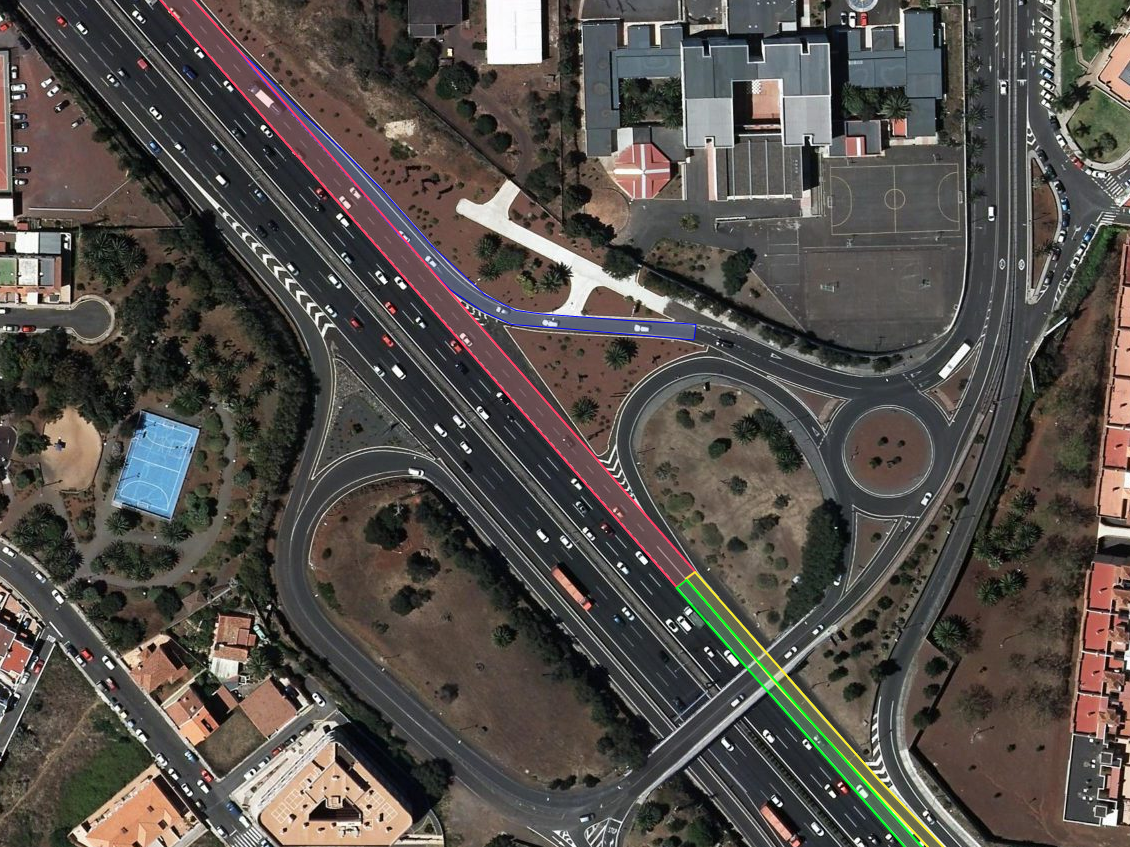
\includegraphics[width=\textwidth]{report/images/salida-tf5-norte-cerca_.png}
      \caption{La misma vista, desde cerca. Permite apreciar los distintos carriles que dan lugar o se incorporan a la salida en cuestión.}
      \label{fig:salida-tf5-norte-cerca}
    \end{subfigure}%
    \caption{La zona roja representa la vía de doble carril (el de la izquierda permite la incorporación a la autopista y también ir a la rotonda de Padre Anchieta, mientras que el derecho permite ir a la rotonda únicamente). La azul se corresponde con la carretera proveniente del IES Viera y Clavijo. El carril verde es el proveniente de la autopista, y el amarillo el proveniente de la rotonda que está por debajo de la autopista. Los tres dan lugar a la vía representada por la zona roja.}
    \label{fig:salida-tf5-norte}
\end{figure}

Bien, la vía representada zona roja (figura~\ref{fig:salida-tf5-norte-cerca}) permite ir a la rotonda o incorporarse a la autopista. Esta incorporación a la TF-5 tiene sentido para los vehículos que vienen de la zona azul o la amarilla. También tendría sentido para los vehículos que provinieran de la autopista (zona verde) que pese a haber tomado la salida deseen reincorporarse a la autopista.

Este comportamiento es el correcto; sin embargo, durante el proceso de conversión \texttt{NETCONVERT} se equivocó y generó un archivo de red que no permitía que los vehículos provenientes de las zonas mencionadas pudieran incorporarse a la TF-5 en dicho lugar (figura~\ref{fig:netedit-tf5-norte-mal}), lo que provocaba que tuvieran que pasar por la rotonda de Padre Anchieta y tomar desde ahí la salida en dirección a la TF-5. Tal comportamiento es indeseable y se corrigió.

\begin{figure}[ht]
    \centering
    \begin{subfigure}[t]{0.48\textwidth}
      \centering
      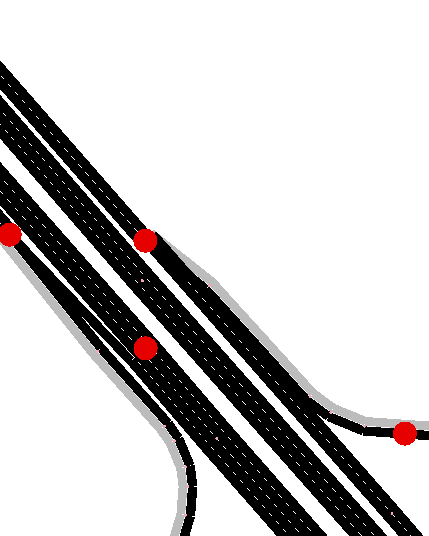
\includegraphics[width=\textwidth]{report/images/netedit-tf5-norte-mal.png}
      \caption{Generación inicial. Véase cómo no es posible la incorporación a la autopista desde los dos carriles que aparecen más a la derecha, que separados de los tres que están en medio (TF-5 dirección norte).}
      \label{fig:netedit-tf5-norte-mal}
    \end{subfigure}
    \hfill
    \begin{subfigure}[t]{0.48\textwidth}
      \centering
      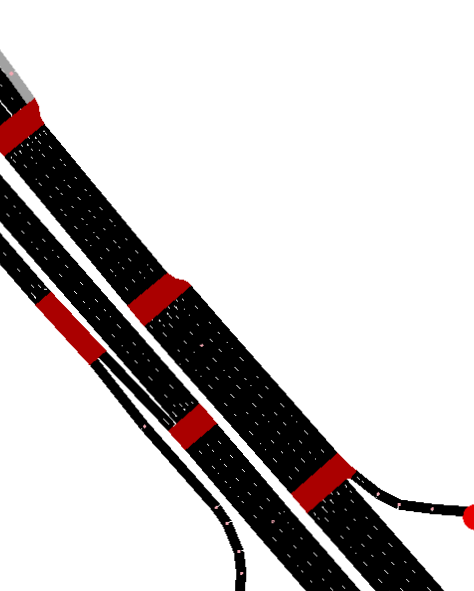
\includegraphics[width=\textwidth]{report/images/netedit.-tf5-norte-bien.png}
      \caption{Modificación realizada. Ahora los vehículos pueden incorporarse a la autopista, pero también los de la autopista pueden tomar la salida más adelante de lo que deberían.}
      \label{fig:netedit-tf5-norte-bien}
    \end{subfigure}%
    \caption{Cambios realizados en la salida de la TF-5 (dir. norte) que va a la rotonda del Padre Anchieta.}
    \label{fig:netedit-tf5-problema}
\end{figure}

Sin embargo, por limitaciones de SUMO, actualmente no es posible establecer carriles con prohibición de cambio asimétrica (como es el caso de la zona roja que se menciona antes): es decir, actualmente no se puede implementar un cambio de carril de modo que sea posible incorporarse a la autopista pero no sea posible realizar la acción inversa. Ello implica que con la modificación realizada para solucionar el problema los vehículos que vayan por la autopista podrán tomar la salida mucho más adelante de lo que en realidad pueden hacerlo (figura~\ref{fig:netedit-tf5-norte-bien}). No obstante, esta solución, aunque imperfecta, es mejor que impedir la incorporación a la TF-5 por los motivos mencionados en el párrafo anterior.

\subsubsection{Otras modificaciones}

Mencionadas las modificaciones más sustanciales, en el archivo de red también se han realizado otras modificaciones menores como la forma de algunas vías (especialmente las vías de la rotonda en sí), que han sido retocadas para que sean más fieles a la realidad; la adición de pasos de peatones, la adición de aceras cuando era necesario y la supresión cuando eran aceras innecesarias o no se correspondían con la realidad, la configuración de los semáforos (de la que se hablará en su propia sección), la corrección de algunas conexiones que permitían giros prohibidos, etc.

\section{Definición de los vehículos y las rutas: el archivo de tráfico}

El principal objetivo a la hora de generar el tráfico y los peatones era hacerlo para una hora de simulación, de modo que dicha hora fuera punta (por ejemplo, a las 8:00 o las 14:00).

En este sentido, varios enfoques han sido tomados en cuenta, resultando al final como ganador la generación de tráfico en función de un algoritmo de maximización del flujo de red, con datos empíricos de aforadores de tráfico provistos por el Cabildo de Tenerife, gracias a un estudio que realizó la entidad en noviembre de 2019 en la rotonda de Padre Anchieta. 

Sin embargo, es relevante mencionar otros enfoques que en durante el desarrollo de este proyecto se tomaron en cuenta, dado que los datos del Cabildo se obtuvieron más adelante durante la fase de desarrollo de este trabajo.

\subsection{Enfoque estocástico}
\label{enfoque_estocastico}

Este enfoque es el más sencillo. Consiste en generar los datos de tráfico y de peatones de forma aleatoria, tanto en flujo como en rutas. SUMO cuenta con una herramienta para hace precisamente esto, \texttt{randomTrips.py}~\cite{noauthor_randomtripspy_nodate}, un script de Python que, con un archivo de red como entrada, permite generar sendos archivos de tráfico y peatones aleatorios.

Las desventajas que plantea este método saltan a la vista: los datos de tráfico generados muy probablemente no se correspondan con la realidad. Esto plantea un problema serio a la hora de obtener una simulación fiel, puesto que los datos de circulación en una situación como la actual pueden afectar sensiblemente al resultado final de la simulación y, en consecuencia, no se podría determinar con fiabilidad si los semáforos son una adición útil o no (que al final es el objetivo último de este trabajo).

A falta de datos de tráfico, este enfoque parece el más aceptable. Sin embargo, el Cabildo de Tenerife publica anualmente un estudio de las intensidades de tráfico en las carreteras de Tenerife~\cite{rodriguez_hernandez_intensidades_2019}. Este estudio no contiene los datos de los aforadores de la rotonda de Padre Anchieta que se mencionaban antes, pero sí contiene la intensidad media diaria (IMD) anual de algunas vías que conectan con la rotonda. La IMD anual de define como el número de vehículos que pasan a través de una sección fija de la carretera dividido entre 365.

Por ejemplo, de las vías que nos interesan el informe contiene los datos de la IMD anual de la TF-5, de la TF-24 (la carretera de La Esperanza) y de la TF-263 (la carretera de Geneto). También tienen datos de la TF-265 (Camino de San Francisco de Paula) pero dicha carretera no conecta directamente con la rotonda, sino que lo hace con la Av. Astrofísico Francisco Sánchez, que sí es una vía de que entra y sale de la rotonda.

Estos datos son extremadamente débiles para inferir el tráfico en una hora particular, sobre todo si queremos el caso de la hora punta de las vías en cuestión. Y eso sin mencionar de que todavía nos faltarían datos de otras vías. Ello nos lleva a plantear el siguiente método.

Sin embargo, este sí fue el enfoque empleado para generar los peatones, puesto que no se dispone de ningún dato sobre los movimientos de las personas que atraviesan los pasos de peatones de las vías de la rotonda.


\subsection{Enfoque de inundación}


\begin{wrapfigure}{L}{5.5cm}
    \centering
    % \captionsetup{width=.8\linewidth}
    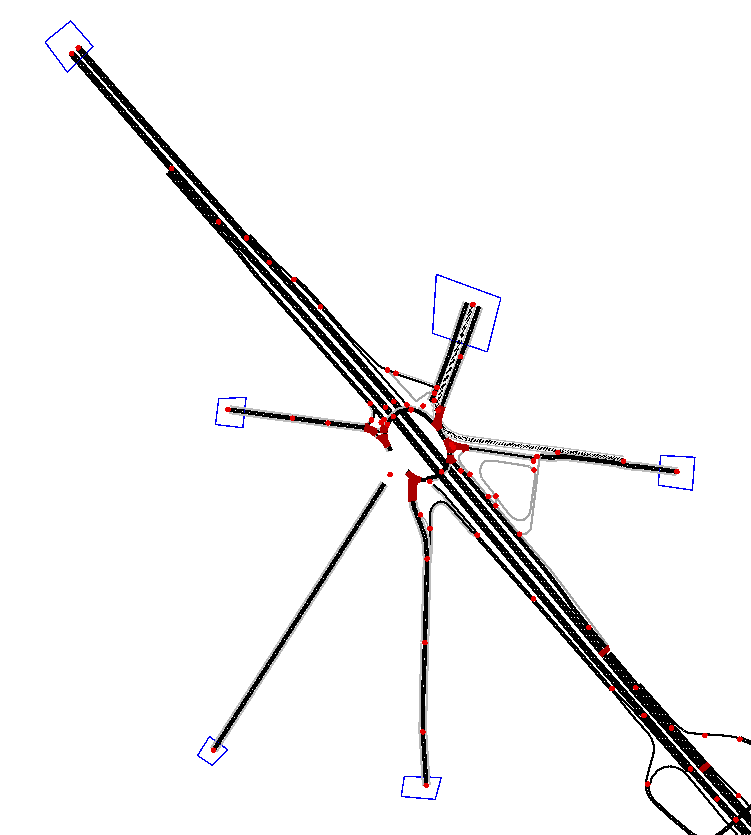
\includegraphics[width=\linewidth]{report/images/taz.png}
    \caption{Las TAZ aparecen delimitadas por las líneas azules.}
    \label{fig:taz}
\end{wrapfigure}


A falta de datos para generar el tráfico, un enfoque interesante residía en generar el tráfico de modo que se lleva al límite el aforo de las vías de la rotonda; es decir, propiciando que circulara el máximo tráfico posible por todas las vías. Este enfoque, aunque en determinados casos resulte irreal, en cierta medida no es tan diferente de lo que sucede en realidad, puesto que en horas punta la rotonda de Padre Anchieta sufre de colas en todas las entradas (en las entradas desde autopista, tanto del norte como del sur, en la Av. Trinidad, en la carretera de la Esperanza y la de Geneto).

Una manera de definir el archivo de tráfico de este enfoque es mediante matrices origen-destino (\textit{O/D matrices})~\cite{otto_anker_nielsen_two_1998}, las cuales se centran en definir el lugar de partida y de llegada junto con el flujo (cantidad de vehículos que circularán desde A hasta B).

Dado que nuestro archivo de red es lo suficientemente pequeño, es viable definir todos los posibles orígenes y destinos de nuestras rutas, asignando un flujo a cada una de ellas lo suficientemente alto como para que pueda haber circulación de vehículos durante una hora.

SUMO viene preparado con una herramienta (\texttt{OD2TRIPS}~\cite{noauthor_od2trips_nodate}) que puede leer archivos de matrices O/D en un formato concreto y convertirlos al formato de archivo de tráfico que nos interesa para realizar la simulación.

La manera en que se definen las matrices O/D viene especificada en~\cite{noauthor_demandimporting_nodate}. La definición de los orígenes se realiza mediante TAZ (\textit{Traffic Analysis Zone}), zonas que se señalan en el archivo de red para agrupar un conjunto de vías de forma que sea fácil establecer el nodo donde se debe iniciar el trayecto y el nodo donde debe finalizar (véase la figura~\ref{fig:taz}).

Este enfoque, como se mencionó antes, solo resultaría útil hasta cierto punto, puesto que solamente representa un estado particular de la rotonda. Generalmente, la rotonda no absorbe el máximo aforo posible en todas las vías, por lo que un enfoque más preciso sería conveniente.

\subsection{Enfoque empírico}

Este enfoque es el que al final se ha empleado, puesto que transcurrido cierto tiempo desde el inicio del proyecto fue posible obtener datos de tráfico correspondientes a 21 aforadores colocados en las inmediaciones de la rotonda, en un estudio realizado por el Cabildo de Tenerife en la semana del 19 al 25 de noviembre de 2019 (véase la figura~\ref{fig:aforadores}). Estos datos vienen desglosados por aforador, día y hora. Los datos de la autopista se obtuvieron desde la web (también del Cabildo)\footnote{La web puede consultarse en \url{http://154.48.153.16:8080/aforos/}}.

\begin{figure}[ht]
    \centering
    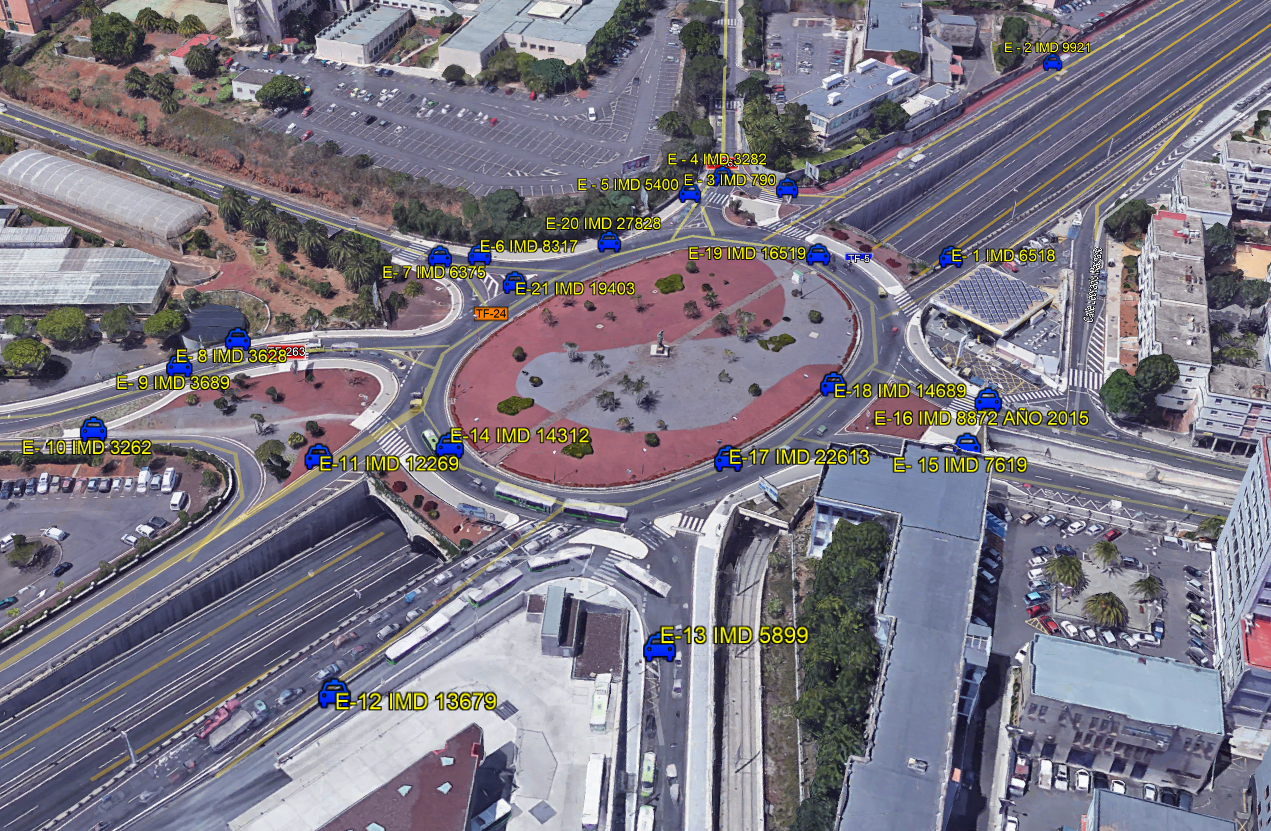
\includegraphics[width=\textwidth]{report/images/aforadores.png}
    \caption{Lugares donde se instalaron los aforadores.}
    \label{fig:aforadores}
\end{figure}

Como nuestro objetivo era simular una hora punta, nos acabamos decantando por obtener los datos del día jueves 21 de noviembre de 2019, a las 8:00, por ser el día que más tráfico hubo a esa hora.

\subsubsection{Generación de rutas: \texttt{flowrouter.py}}

Tener los datos de los aforadores es una gran ayuda a la hora de estimar con fiabilidad el tráfico real de la rotonda, pero no lo es todo, puesto que no indica qué ruta han seguido dichos vehículos ni tampoco cuál es el destino al que habían de llegar. Es decir, es conocido cuántos coches salen de A y cuántos llegan a B, pero no conocemos cuáles de los coches que han llegado a B procedían de A. Al final, de lo que disponemos es de contadores de vehículos, pero lo que nos interesa son las rutas que siguen dichos vehículos; o sea, una matriz O/D.

Así pues, el problema de inferir una matriz O/D a partir de datos de contadores de tráfico no es en absoluto desconocido y abunda bastante literatura sobre cómo abordar este problema (véase~\cite{otto_anker_nielsen_two_1998}). 

Sin embargo, y como no podía ser de otro modo, los creadores de SUMO ya habían previsto que esta situación podría darse, así que decidieron incorporar dos herramientas para calcular las rutas con sus respectivos flujos a partir de datos de aforadores: \texttt{DFROUTER}~\cite{noauthor_dfrouter_nodate}; y su versión mejorada, \texttt{flowrouter.py}~\cite{noauthor_flowrouterpy_nodate,behrisch_route_2018}, la cual ha sido finalmente la empleada para generar el tráfico.

La diferencia entre ambas radica en el algoritmo que emplean para calcular las rutas y los flujos de los vehículos. \texttt{DFROUTER} está pensada para redes en las cuales todas las posibles entradas y salidas cuentan con aforadores, y los datos que estos brindan son relativamente precisos. \texttt{flowrouter.py}, por otro lado, está pensado para trabajar con más incertidumbre y, por tanto, es capaz de lidiar con redes en las cuales faltan aforadores y donde los datos pueden presentar cierto nivel de inconsistencia.

Estas herramientas toman como entrada tres archivos:

\begin{itemize}
    \item El archivo de red.
    \item Un archivo con los datos de los aforadores (nombre, posición, y si es de origen, destino o está <<en medio>> ---esta clasificación, tal y como se infiere de su nombre, está reservada para aforadores que no son clasificables como de origen o destino---).
    \item Datos de flujo (aforador, flujo, plazo durante el cuál se detectó dicho flujo, etc.).
\end{itemize}

Y como salida general dos archivos:

\begin{itemize}
    \item Un archivo de rutas.
    \item Un archivo de flujos (definidos en función de las rutas).
\end{itemize}

Ha de señalarse que ambas herramientas están pensadas para trabajar con redes relativamente simples, concretamente autopistas, dado que suelen estar bien dotadas de aforadores y no poseen una topología especialmente compleja; por lo que es posible que los resultados que brindan dichas herramientas a veces pueden ser erráticos y confusos, por lo que la entrada debe ser lo más completa y precisa posible.

Durante una prueba inicial, los resultados obtenidos con \texttt{flowrouter.py} mostraban que había rutas que no seguía ningún vehículo cuando realmente debía de haber algún flujo. También, en algunos casos, se generaban rutas ilógicas, como circular desde la carretera de Geneto con la intención de incorporarse a la TF-5 sentido sur pasando por la rotonda, ignorando el desvío (más corto) del que dispone la carretera, que permite incorporarse a la autopista directamente.

Es muy posible que este tipo de errores e inexactitudes se produjeran por la intención del algoritmo de satisfacer las restricciones impuestas por los datos de los aforadores. Asimismo, la configuración de algunos de estos contadores no era la idónea. 

Por ejemplo, volviendo al caso de la carretera de Geneto, según muestra la figura~\ref{fig:aforadores}, esta cuenta con tres aforadores: el E-8 (en sentido ascendente), el E-9 (en sentido descendente) y el E-10 (en sentido descendente, colocado en el desvío hacia la autopista).

Se da la circunstancia de que, por la manera en que \texttt{flowrouter.py} calcula las rutas, es posible que designara los orígenes y los destinos en unos nodos en los cuales realmente no deseamos que acabe el tráfico (porque, por ejemplo, no daría tiempo a que se formaran colas o a apreciar mejor durante la simulación el funcionamiento del tráfico).

Todos estos problemas se solucionaron (en su mayoría) añadiendo nuevos contadores manualmente. Para el ejemplo que estamos tratando, bastó con añadir un contador en la carretera de Geneto, sentido descendente, que estuviera un poco más arriba y que sumara el flujo de los contadores E-9 y E-10, y colocando a la misma altura el contador E-8 (el que estaba en sentido ascendente). Hecho con el resto de vías, la generación del tráfico es menos errática y durante la simulación es posible apreciar mejor el flujo de los vehículos.

Este método es, pues, el que mejor resultados ha brindado y es con el que finalmente se llevó a cabo la generación del tráfico.
\chapter{Simulación y optimización}
\label{cap:simulacion}

\section{Configuración de las instancias empleadas para la simulación del tráfico}

\subsection{Instancias sin semáforos}

Actualmente, la rotonda de Padre Anchieta no cuenta con ningún semáforo. La regulación del tráfico se produce únicamente por dos factores: la señalización (señales de ceda el paso, principalmente) y los pasos de peatones, los cuales hemos tenido en cuenta a la hora de evaluar el comportamiento del tráfico.

Asimismo, la simulación de estas instancias realizaría una función de control con respecto a las instancias con semáforos, puesto que nos permitiría comparar el rendimiento de la rotonda actual con el caso de que tuviera semáforos.

Se proponen tres instancias sin semáforos:

\paragraph{S\textsubscript{1} --- <<anchieta\_no\_tls>>.} Es la instancia más sencilla, puesto que únicamente se simulará tráfico rodado sin tener en cuenta a los peatones.


\paragraph{S\textsubscript{2} --- <<anchieta\_no\_tls\_few\_pedestrians>>.} Esta instancia es exactamente igual a la anterior, pero cuenta con aproximadamente 500 peatones generados con \texttt{randomTrips.py} mencionada en la sección~\ref{enfoque_estocastico}.


\paragraph{S\textsubscript{3} --- <<anchieta\_no\_tls\_many\_pedestrians>>.} De nuevo, esta instancia es idéntica a las dos primeras, con la salvedad de que cuenta con aproximadamente 2000 peatones generados con la misma herramienta, \texttt{randomTrips.py}.


Tal y como se mencionó en la sección~\ref{enfoque_estocastico}, la generación de los peatones es completamente aleatoria y distribuida uniformemente tanto en tiempo (una hora de simulación) como en espacio, puesto que desafortunadamente no existen datos lo suficientemente granulares sobre los movimientos de los peatones en la zona.


\subsection{Instancias con semáforos}
\label{subsec:instancias}

Definidas las instancias anteriores, llega el momento de tomar una decisión importante: ¿dónde han de situarse los semáforos? A fin de cuentas, la rotonda de Padre Anchieta no es una zona que contara previamente con semáforos, por lo que nos corresponde a nosotros determinar la localización de estos.

Así pues, se proponen cuatro instancias con configuraciones semafóricas distintas:

\paragraph{S\textsubscript{4} --- <<anchieta\_tls\_interior\_lane\_always\_green>>.} Semáforos en cada entrada y salida, con el carril interior siempre en verde. Una posible configuración de los semáforos es añadir uno en cada entrada y salida de la rotonda, de modo que esté absolutamente regulada por estos. Además, el carril interior permanecería en verde siempre que fuera posible, cambiando de color únicamente en los casos en los que la vía entrada a la rotonda tenga dos carriles y sea necesario regular el paso entre los carriles izquierdos de la entrada y la rotonda. Esta instancia no necesita simular ningún peatón, puesto que todas las entradas y salidas estarían reguladas por semáforos y, por extensión, también los pasos de peatones. Ello hace innecesario evaluar cómo se comportarían los peatones durante la simulación (simplemente se quedarían parados mientras el semáforo peatonal cambia a verde para que puedan cruzar).

\paragraph{S\textsubscript{5} --- <<anchieta\_tls\_interior\_lane\_changes>>.} Semáforos en cada entrada y salida, con el carril interior cambiando de color. Es la misma configuración que la 1, con la salvedad de que el carril interior cambia de color junto con el exterior independientemente de que la entrada que se esté regulando tenga un carril o dos. El objetivo de simular estas dos configuraciones es comprobar cuál es más eficiente gestionando el carril interior. Véase la Figura~\ref{fig:conf2}. Tanto en esta configuración como en la anterior, las fases se modificaron manualmente para garantizar que siguen un ciclo correcto. Esta instancia tampoco tiene en cuenta los peatones por los mismos motivos que la anterior.

\paragraph{S\textsubscript{6} --- <<anchieta\_tls\_few\_pedestrians>>.} Semáforos al norte y al sur de la rotonda con pocos peatones. Este caso particular solamente instala dos semáforos: uno al norte de la rotonda (entre la entrada de la TF-5 en sentido Santa Cruz y la salida hacia la TF-5 en sentido La Orotava) y otro al sur (entre la salida hacia la TF-5 en sentido Santa Cruz y la entrada de doble carril desde la TF-5 en sentido La Orotava). Véase la Figura~\ref{fig:conf3}. Esta instancia, dado que cuenta con pasos de peatones sin regular por semáforos, sí tendrá en cuenta durante la simulación a los peatones, cuya cantidad y rutas han sido definidas aleatoriamente por \texttt{randomTrips.py} dado que no existen datos medidos sobre tránsito de peatones en la zona. Esta instancia cuenta, aproximadamente, con 500 peatones.

\paragraph{S\textsubscript{7} --- <<anchieta\_tls\_many\_pedestrians>>.} Semáforos al norte y al sur de la rotonda con muchos peatones. Esta instancia es idéntica a la anterior, con la salvedad de que se ha cuadruplicado la cantidad de peatones que circulan por la zona, para poder evaluar la circulación de los vehículos con un tránsito más denso de peatones.


\begin{figure}[ht]
    \centering
    \begin{subfigure}[t]{0.48\textwidth}
        \centering
        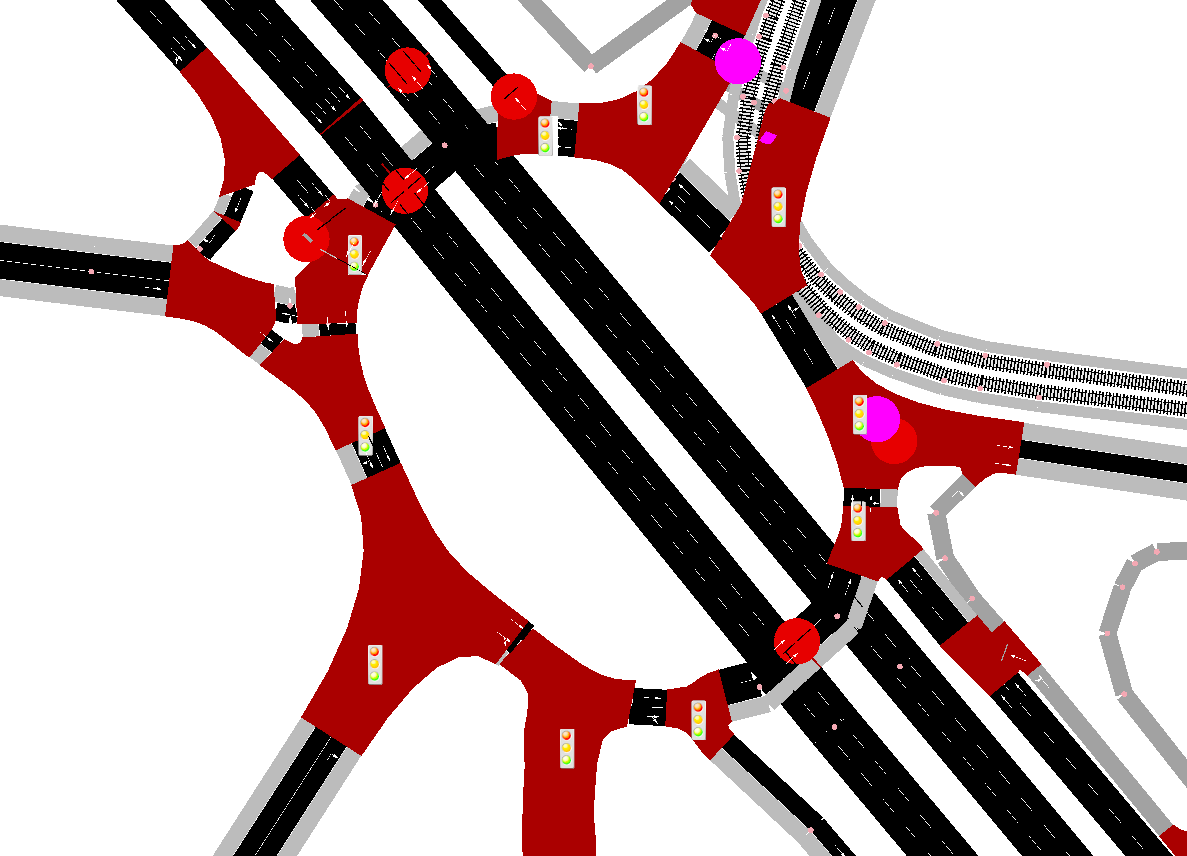
\includegraphics[width=\textwidth]{report/images/conf2.png}
        \caption{Imagen del archivo de red con los semáforos de las configuraciones S\textsubscript{4} y S\textsubscript{5}.}
        \label{fig:conf2}
    \end{subfigure}
    \hfill
    \begin{subfigure}[t]{0.48\textwidth}
        \centering
        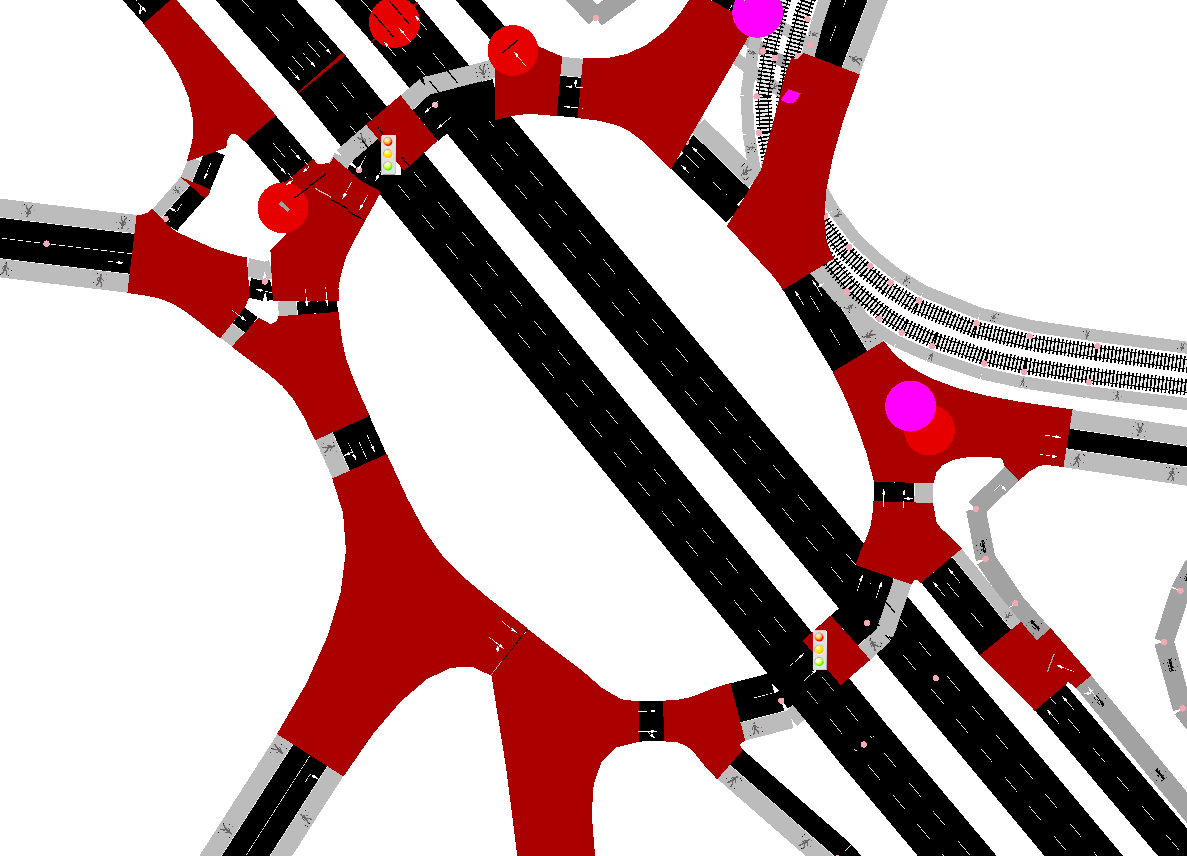
\includegraphics[width=\textwidth]{report/images/conf3.png}
        \caption{Imagen del archivo de red con los semáforos de la configuración S\textsubscript{6} y S\textsubscript{7}.}
        \label{fig:conf3}
    \end{subfigure}
    \caption{Distintas configuraciones de los semáforos.}
    \label{fig:confs}
\end{figure}



\section{El algoritmo evolutivo}

Una vez se han definido los archivos de la simulación, corresponde evaluar la manera en que se va a implementar el algoritmo evolutivo. Para esto se ha empleado \texttt{Genetics.js}, una librería programada en TypeScript orientada a algoritmos evolutivos; en particular, algoritmos genéticos. Esta librería la programó Cristian Abrante, un antiguo alumno de la Escuela Superior de Ingeniería y Tecnología, para su TFG titulado <<Framework web de computación evolutiva>>~\cite{abrante_dorta_framework_2019}. 

Antes de proceder a emplear la librería, se hizo un fork de la misma y se realizaron algunos cambios. Los principales cambios están relacionados con la importación de módulos en TypeScript, de modo que todas las clases y elementos necesarios se pudieran importar directamente desde \texttt{genetics-js}. Asimismo, se modificó la librería para que los valores que el generador de números aleatorios que emplea el algoritmo pudiera detectar para qué fase en concreto estaba generando el valor, de modo que si cualquier fase contenía un semáforo en amarillo su duración sería exactamente de cuatro segundos.

\subsection{Genotipo y fenotipo: representación de las posibles soluciones}

En un algoritmo evolutivo (AE) es importante distinguir dos conceptos: el fenotipo y el genotipo.

\textbf{El fenotipo} es el conjunto de objetos o entidades que conforman las posibles soluciones del problema original~\cite{eiben_introduction_2003}. Para el caso que aquí nos concierne, se trataría de las duraciones de las fases de cada uno de los semáforos de las intersecciones que figuran en el archivo de red.

Pensemos en una sencilla intersección entre dos calles de un solo carril, estando regulada dicha intersección por dos semáforos (uno en cada calle), según muestra la Figura~\ref{fig:semaforo-simple}.

\begin{figure}[ht]
    \centering
    \begin{subfigure}[t]{0.32\textwidth}
        \centering
        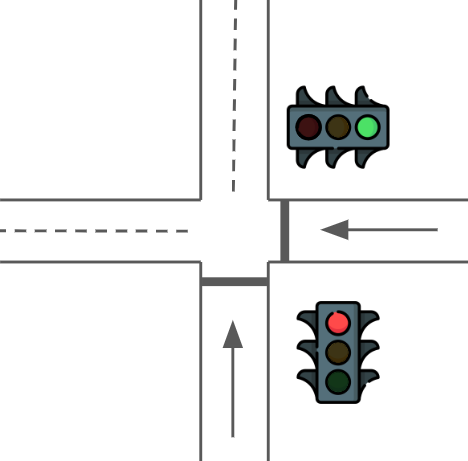
\includegraphics[width=\textwidth]{report/images/semaforossimple1.png}
        \caption{Fase 1.}
        \label{fig:semaforo-simple-1}
    \end{subfigure}
    \hfill
    \begin{subfigure}[t]{0.32\textwidth}
        \centering
        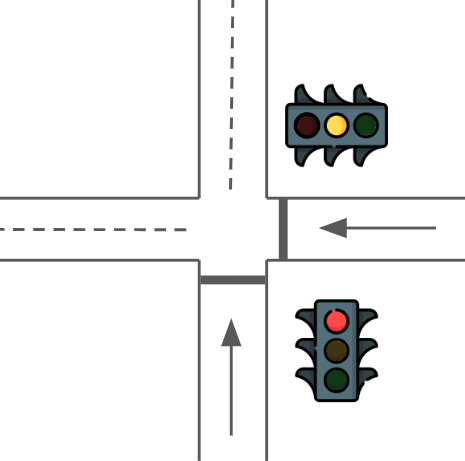
\includegraphics[width=\textwidth]{report/images/semaforossimple2.png}
        \caption{Fase 2.}
        \label{fig:semaforo-simple-2}
    \end{subfigure}
    \hfill
    \begin{subfigure}[t]{0.32\textwidth}
        \centering
        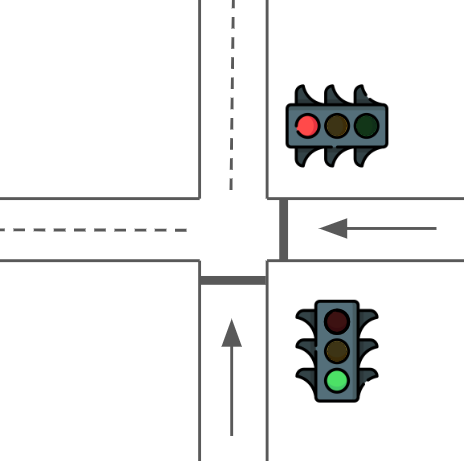
\includegraphics[width=\textwidth]{report/images/semaforossimple3.png}
        \caption{Fase 3.}
        \label{fig:semaforo-simple-3}
    \end{subfigure}
    \caption{Cambio de fases en una intersección.}
    \label{fig:semaforo-simple}
\end{figure}

Cada una de las fases de esta intersección tienen una duración asignada. Por ejemplo, podríamos asignar una duración a la fase 1 (Figura~\ref{fig:semaforo-simple-1}) podría de 30 segundos, mientras que la 2 (Figura~\ref{fig:semaforo-simple-2}) duraría 4 segundos (dado que es una fase que contiene un semáforo en ámbar), y finalmente la fase 3 duraría 45 segundos. Este conjunto de duraciones es una posible solución a nuestro problema, que al final lo que busca es asignar las duraciones a las fases de los semáforos de modo que permitan circular al tráfico de la manera más eficiente, y es con lo que lidiaría el algoritmo evolutivo. Así es, pues, como se representa el fenotipo.

\textbf{El genotipo}, por otro lado, es la codificación de nuestra solución, es la manera en que representamos los individuos de modo que el algoritmo evolutivo pueda trabajar con ellos. Para el caso en cuestión, el fenotipo mostrado por la Figura~\ref{fig:semaforo-simple} lo representaríamos por un \textit{array} de valores que se corresponderían con las duraciones de dichas fases. Por ejemplo: \texttt{[30, 4, 45]}. Suponiendo que contásemos con varias intersecciones, cada una de ellas compuesta de varios semáforos, y cada uno de estos compuestos de varias fases con sus respectivas duraciones, simplemente se añadirían al \textit{array} dichas duraciones como valores numéricos igual que antes: \texttt{[30, 4, 45, 20, 55, 4, 80, 22, 47, 4, ...]}.

Vale la pena mencionar que, además de lidiar con duraciones de fases, el \textit{array} también contendrá valores numéricos en representación de los retardos de las intersecciones (véase la Figura~\ref{fig:genotipo}). Estos retardos son los que se emplean para sincronizar varias intersecciones con semáforos de modo que se produzcan las denominadas \textit{oleadas de verde}~\cite{segredo_optimising_2019}.


\begin{figure}[ht]
    \centering
    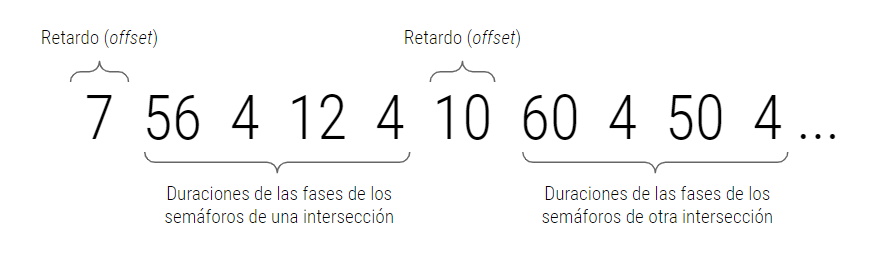
\includegraphics[width=\textwidth]{report/images/genotipo.png}
    \caption{Ejemplo de genotipo.}
    \label{fig:genotipo}
\end{figure}


\subsection{Función objetivo}
\label{subsec:funcion}

Una vez definidos los individuos con los que se va a trabajar, es necesario establecer una función que determine que tan buenos candidatos son. Así pues, se propone una función objetivo adaptada del artículo~\cite{segredo_optimising_2019} y que toma en cuenta los siguientes objetivos:

\begin{itemize}
    \item Ha de maximizarse el número de vehículos $V_R$ que llegan a su destino; de manera equivalente, ha de minimizarse la cantidad de vehículos $V_{NR}$ que no llegan a su destino en un determinado tiempo de simulación $T_{sim}$.
    \item Ha de minimizarse la duración general media del trayecto de todos los vehículos $T_{trip}$.
    \item Ha de minimizarse el tiempo total $T_{sw}$ que han perdido los vehículos por estar parados o por ir más lento de lo que quisieran.
\end{itemize}

Todos los objetivos anteriores se combinan en la siguiente función objetivo:

$$
f_{obj} = \frac{V_R^2}{T_{trip} + T_{sw} + V_{NR} T_{sim}}
$$

Como puede apreciarse, los objetivos de maximización están colocados en el numerador; y los de minimización, en el denominador. Por ello, la función propuesta es de maximización. Esta es una de las diferencias respecto de la función que se adapta del artículo de referencia; principalmente porque la librería Genetics.js empleada no admite plantear el problema como uno de minimización. Otra de las diferencias radica en que la función propuesta no tiene en cuenta la maximización de la duración de las fases que contengan más semáforos en verde que en rojo.

Al igual que en la función objetivo de referencia, la que se propone para este proyecto eleva al cuadrado el término $V_R$ para darle prioridad sobre el resto, dado que es el objetivo más importante (que los vehículos completen su trayecto). Además, $V_{NR}$ se multiplica por $T_{sim}$ para penalizar el incremento de vehículos que no alcanzan su destino en función del tiempo de la simulación.

\section{Aplicación del algoritmo y estudio estadístico sobre los parámetros óptimos de ejecución}

Con el objetivo de mejorar el funcionamiento del algoritmo y saber que se están empleando los parámetros adecuados de configuración para obtener los mejores resultados, se ha realizado un estudio estadístico que alterna distintos parámetros del algoritmo evolutivo.

Este estudio se ha realizado por separado para cada una de las instancias detalladas en la sección~\ref{subsec:instancias}, dado que son las únicas que requieren el empleo del algoritmo.

\subsection{Parámetros de configuración}
\label{subsec:parametros}

Las variables tenidas en cuenta para el estudio estadístico han sido dos:

\textbf{Cruce} \textit{(Crossover)}. A la hora de evaluar el cruce entre genotipos, se han valorado dos opciones: \texttt{OnePointCrossover} y \texttt{UniformCrossover}.

\begin{itemize}
    \item \texttt{OnePointCrossover}~\cite{eiben_422_2003} intercambia un único punto (situado en la misma posición) de ambos genotipos. Por ejemplo: supongamos que manejamos dos genotipos distintos, los cuales podemos representar en binario: 0000 y 1111. Este operador de cruce seleccionará una posición aleatoria, la cual será la misma para ambos genotipos, y dividirá a cada uno en dos partes distintas. A continuación, intercambiará entre ambos genotipos las mitades de uno de los lados. En el caso del genotipo anterior, si la posición seleccionada es la correspondiente al segundo elemento de izquierda a derecha, el resultado después del cruce sería 0011 y 1100 para el primer y el segundo genotipo, respectivamente.
    \item \texttt{UniformCrossover}~\cite{eiben_422_2003}, por otro lado, intercambia elementos individuales entre sí cuyas posiciones son seleccionadas aleatoriamente en función de un umbral, que determina la probabilidad de que se produzca dicho intercambio. Tomando los genotipos anteriores, 0000 y 1111, y un umbral de 0.50, un posible resultado de aplicar el cruce podría ser 1001 y 0110 para el primer y segundo genotipo, respectivamente. Véase como, en este ejemplo ideal, un 50 \% de los puntos han sido intercambiados entre sí, en consonancia con el umbral definido. Evidentemente, si el umbral es mayor, una mayor cantidad de puntos serán intercambiados entre sí, y viceversa.
\end{itemize}


\textbf{Población} \textit{(Population)}. La población determina la cantidad de individuos que son evaluados durante una generación. En particular, se han seleccionado dos valores: 10 y 50.

Junto con las variables mencionados, el algoritmo evolutivo se ha ejecutado, para el estudio estadístico, con los siguientes parámetros:

\begin{itemize}
    \item Generaciones: 50. 
    \item Selección: \texttt{RouletteWheel}~\cite{lipowski_roulette-wheel_2012}. Este método selecciona los mejores candidatos a la vez que ofrece a aquellos individuos con peor fitness que también sean escogidos. Para ello, asigna a cada individuo una probabilidad de ser seleccionado de manera proporcional a su fitness.
    \item Mutación: \texttt{RandomResseting}~\cite{abrante_dorta_framework_2019}. Selecciona de manera uniforme un gen del individuo y le asigna un valor aleatorio dentro del rango $[4,120]$. Sin embargo, seleccionará siempre el valor $4$ cuando el gen a mutar sea de una fase que contiene un semáforo en fase ámbar. La cantidad de genes que serán mutados viene determinada por el ratio de mutación $r$, que para este proyecto equivale a $1 / g$, donde $g$ la cantidad de genes.
    \item Condición de terminación: por generaciones.
\end{itemize}


Con respecto a la simulación, se han tenido en cuenta los siguientes parámetros:

\begin{itemize}
    \item Duración de la simulación: 1800 segundos (30 minutos, tramo 8:00-8:30).
    \item Tiempo para teletrasporte: 120 segundos. Este valor determina el tiempo que tardará el simulador antes de teletransportar un vehículo que, por razones estocásticas, del funcionamiento del simulador y de cómo está configurada la red, puede haberse quedado estancado.
\end{itemize}


\subsection{Proceso del estudio estadístico}
\label{subsec:proceso-estudio}

Este estudio se centra en analizar si existe algún tipo de diferencia estadística en los resultados de emplear unos parámetros u otros, de modo que al final se empleasen los que mejor resultado devolvieran. Para este estudio se han tenido en cuenta dos parámetros: cruce y tamaño de población, para cada una de las  cuatro instancias citadas en la sección~\ref{subsec:instancias}.

Contando con que tenemos 4 instancias que simular, y dado que para cada una de ellas hay 2 variables, cada una de ellas con 2 posibles valores, en total han de realizarse 16 ejecuciones en total: la primera instancia con una población de 10 individuos y usando un cruce tipo \texttt{OnePointCrossover}, la misma instancia pero variando el cruce, luego variando la población, y luego ambos; y de igual modo para el resto de las instancias.

Además, en aras de unos resultados más robustos, cada una de las 16 configuraciones se ha ejecutado 10 veces con semillas distintas, para evitar que pudiera derivarse algún tipo de sesgo e introducir aleatoriedad en la simulación, algo que sucede en la vida real puesto que no hay dos días en que todos los vehículos y peatones realicen exactamente la misma ruta en el mismo momento. En cada una de esas ejecuciones también han de contarse las generaciones y los individuos de cada una de estas, puesto que cada individuo obtiene su valor de fitness a partir de los resultados de la simulación. Así pues, dado que todas las ejecuciones han tenido como parámetro 50 generaciones, y dado que la mitad de las 16 configuraciones empleaban 10 individuos y la otra mitad 50, el cúmulo de simulaciones realizadas se eleva a las 240.000.

$$
S = \sum_{1}^{i} C_i * G * I_i * E
$$

donde $S$ es el número de simulaciones realizadas, $i$ es la cantidad de valores seleccionados para el tamaño de la población (en este caso, 10 y 50, por lo que $i=2$), $C_i$ equivale a la cantidad de configuraciones que empleaban $I_i$ individuos (de las 16 configuraciones, la mitad empleaba 10 y la otra 50, por lo que $A_1 = A_2 = 8$), $G$ es la cantidad de generaciones (50, igual en todos los casos) y $E$ la de ejecuciones (10, es un valor fijo). Sentado lo anterior:

$$
S = (8*50*10*10) + (8*50*50*10) = 240.000
$$

Dado que cada una de las ejecuciones dura aproximadamente 30 segundos, el tiempo estimado (suponiendo que se ejecutasen secuencialmente) para completar el estudio es de aproximadamente 2000 horas (83 días). Por suerte, se ha contado con un ordenador considerablemente más potente para llevar a cabo el estudio, reduciendo el tiempo de simulación a dos días.

Para determinar qué conjunto de parámetros es mejor para una instancia particular, el algoritmo ejecutado para llevar a cabo el estudio estadístico evalúa dos posibles conjuntos entre sí para determinar de ellos cuál es mejor. Como hemos visto antes, hay 2 parámetros (recordemos, cruce y cantidad de individuos por generación; llamémosles $P_{1x}$ y $P_{2x}$) con 2 posibles valores cada uno, lo cual representamos con la $x$. Así pues, podríamos contar con que tenemos $P_{11}$, $P_{12}$, $P_{21}$ y $P_{22}$ conjuntos de parámetros que estamos valorando para cada instancia; dónde, por ejemplo, $P_{11}$ equivale a \texttt{OnePointCrossover} y 10 individuos. 

Bien, el algoritmo evaluará los resultados que ofrece emplear el conjunto $P_{11}$ contra $P_{12}$, luego contra $P_{21}$; y así sucesivamente. Cuando haya terminado de evaluar dicho conjunto, continuará evaluando el siguiente ($P_{12}$) contra el resto salvo el primero, y así hasta que todas las combinaciones (sin repeticiones) de parejas posibles hayan sido comparadas entre sí.

Para determinar cuándo hay una diferencia estadística entre un conjunto u otro el algoritmo recibe como entrada dos vectores de valores (uno por conjunto de parámetros) a los cuales se les aplican varios tests estadísticos. A dichos vectores los denominaremos $\vec{Q}_x$.

Cada vector contiene 10 valores, uno por cada ejecución. Cada una de las ejecuciones del algoritmo se ha llevado a cabo con 50 generaciones. Para determinar el valor de un elemento del vector, se ha seleccionado el valor de fitness del mejor individuo de cada una de las 50 generaciones y se ha realizado la media. Así pues, en cada vector tenemos las medias del fitness de los mejores individuos por generación de cada ejecución.

Luego, una vez que contamos con ambos vectores, se les aplica el test de Shapiro para determinar el p-value de cada conjunto. Si algún p-value es menor a 0.05, se pasa directamente al test de Kruskal Wallis; si no, ambos p-value son mayores a 0.05, por lo que se cumple el test de normalidad y se ejecuta el test de Levene para analizar las varianzas entre ambos conjuntos. Si dicho test devuelve un resultado mayor a 0.05, las varianzas no presentan una diferencia significativa y por tanto el p-value final se calcula con el test de Anova. En caso de que las varianzas sí presenten una diferencia significativa, dicho p-value se calcula con el test de Welch.

Una vez que hemos pasado la serie de tests anteriores, tendremos un p-value final. Si es superior a 0.05, se asume que no hay diferencia entre aplicar uno u otro conjunto puesto que ambos ofrecerán el mismo resultado; pero si es inferior a 0.05 existe una diferencia estadística entre ambos conjuntos de parámetros y, para determinar cual es mejor, se selecciona el que tenga mayor mediana calculada a partir de los elementos del vector $\vec{Q}_x$ del conjunto.

Los resultados de este estudio se comentarán en su respectiva sección en el capítulo siguiente.
\chapter{Resultados}
\label{cap:4-resultados}

\section{Estudio estadístico}

Esta sección presenta los resultados fruto de realizar el estudio estadístico, con el objetivo de averiguar cuales eran los mejores parámetros de los propuestos en el capítulo anterior para que el algoritmo evolutivo consiguiera mejores resultados. Se evalúa cada instancia de las mencionadas en la sección~\ref{subsec:instancias} por separado, aportando un conjunto de gráficas de la evolución del fitness para cada conjunto de parámetros evaluado y una tabla con los resultados numéricos de la comparación entre sí de todos los conjuntos, para averiguar si existe una diferencia estadística en los resultados ofrecidos.

\subsection{Instancia S\textsubscript{4}: <<anchieta\_tls\_interior\_lane\_always\_green>>}


Con respecto a los resultados del estudio estadístico de la primera instancia, se puede comprobar en la Figura~\ref{fig:estudio:anchieta_tls_interior_lane_always_green} la evolución del fitness para cada una de las cuatro configuraciones que se plantearon para la instancia. 

Las gráficas revelan claramente un incremento del fitness cuando la población es de 50 individuos, independientemente del cruce empleado, pese a que la mejoría no es especialmente abundante. Así pues, para determinar cual configuración es la mejor, hay que referirse a la Tabla~\ref{tab:estudio:anchieta_tls_interior_lane_always_green}. Aquí figuran todas las configuraciones enfrentadas entre sí en parejas.

En dicha tabla se puede apreciar como, al enfrentar a las configuraciones entre sí, la combinación de cruce \texttt{UniformCrossover} y población 50 se coloca como la mejor de todas, puesto que <<ganó>> tres de los <<enfrentamientos>> contra el resto de las configuraciones, revelándose así como el conjunto de parámetros del algoritmo evolutivo que ofrecen mejores resultados. En segunda posición queda el conjunto \texttt{OnePointCrossover} y población 50, al haber ganado solo dos de los enfrentamientos. Finalmente, puede apreciarse como no existe ninguna diferencia en emplear una configuración que tenga 10 individuos con cualquier tipo de cruce.


\begin{figure}[h]
    \centering
    \begin{subfigure}[t]{.49\textwidth}
      \centering
      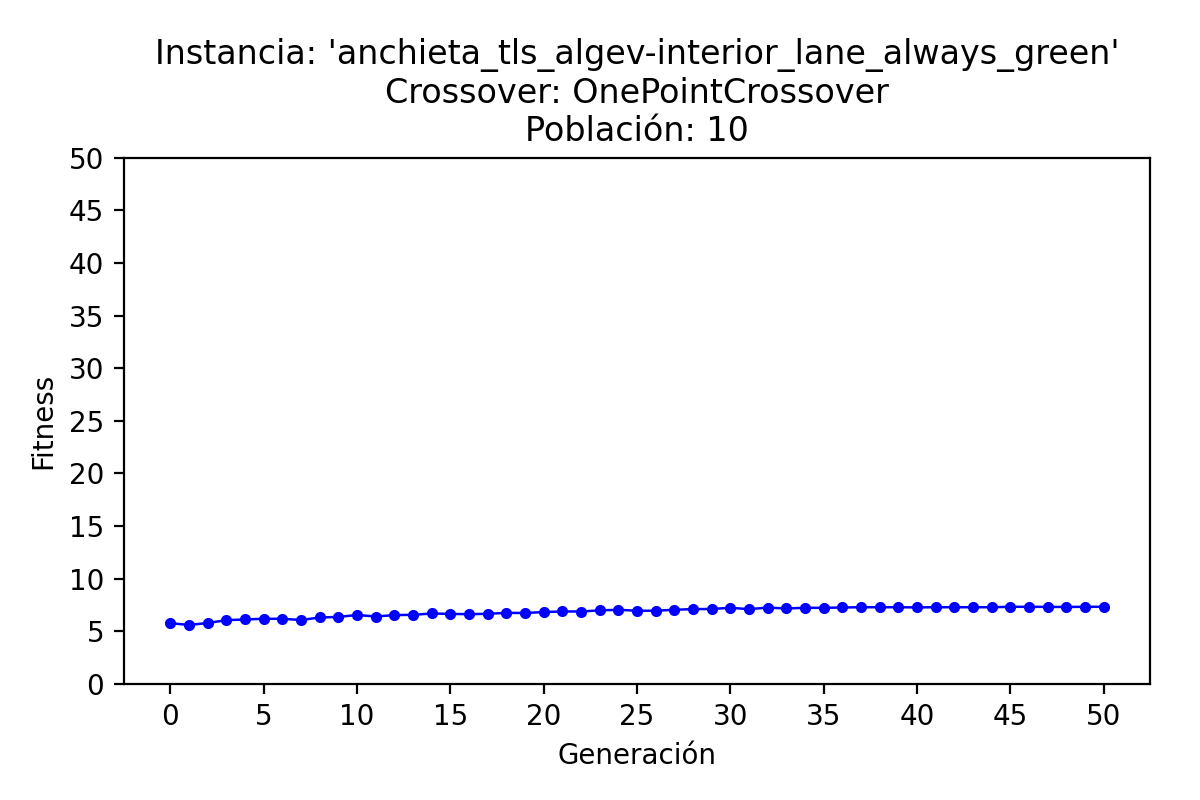
\includegraphics[width=\textwidth]{report/images/estudio/anchieta_tls_algev-interior_lane_always_green-OnePointCrossover-10.png}
    \end{subfigure}
    \hfill
    \begin{subfigure}[t]{.49\textwidth}
      \centering
      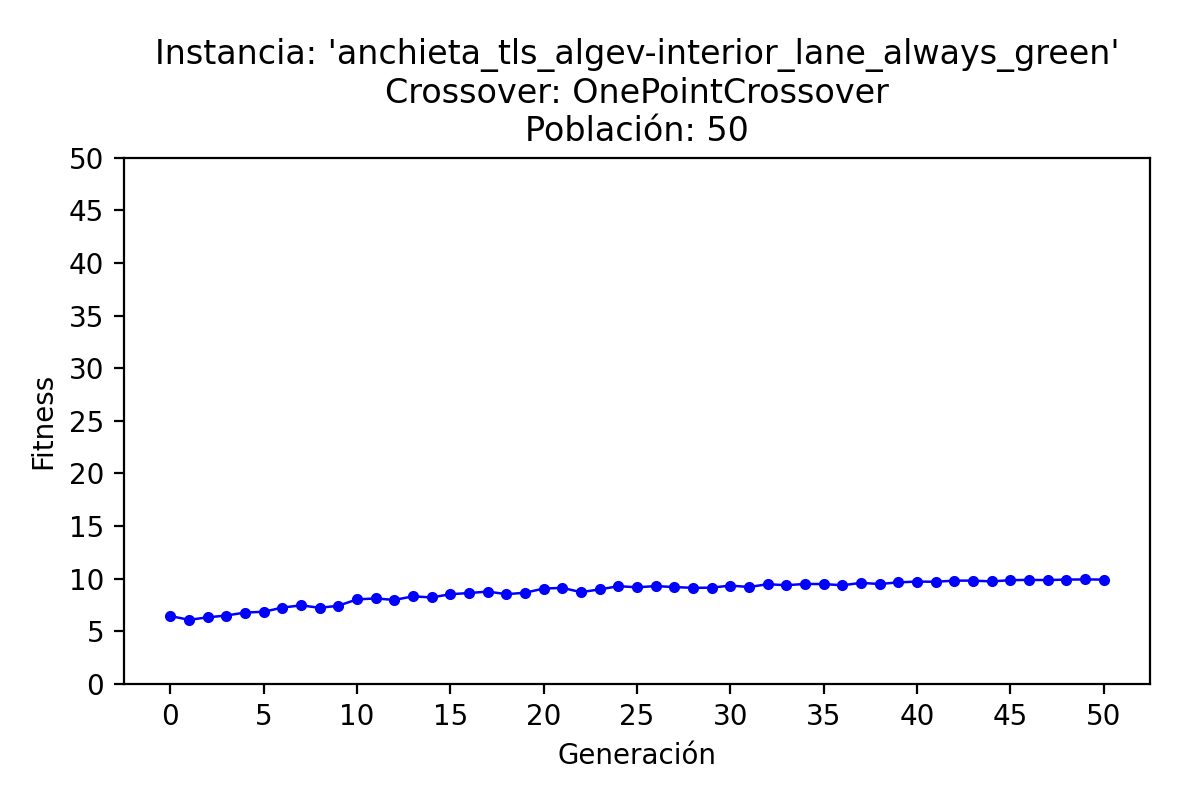
\includegraphics[width=\textwidth]{report/images/estudio/anchieta_tls_algev-interior_lane_always_green-OnePointCrossover-50.png}
    \end{subfigure}
    \vspace{0.7cm}
    \begin{subfigure}[t]{.49\textwidth}
      \centering
      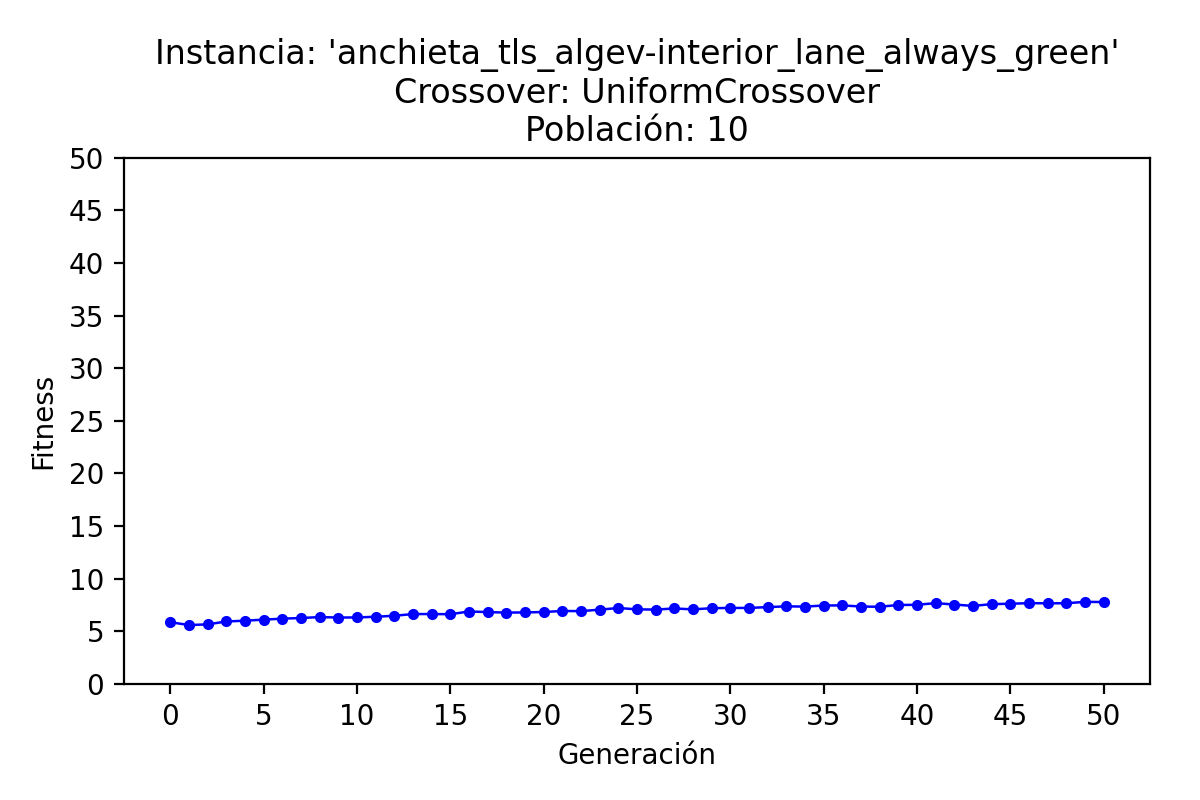
\includegraphics[width=\textwidth]{report/images/estudio/anchieta_tls_algev-interior_lane_always_green-UniformCrossover-10.png}
    \end{subfigure}
    \hfill
    \begin{subfigure}[t]{.49\textwidth}
      \centering
      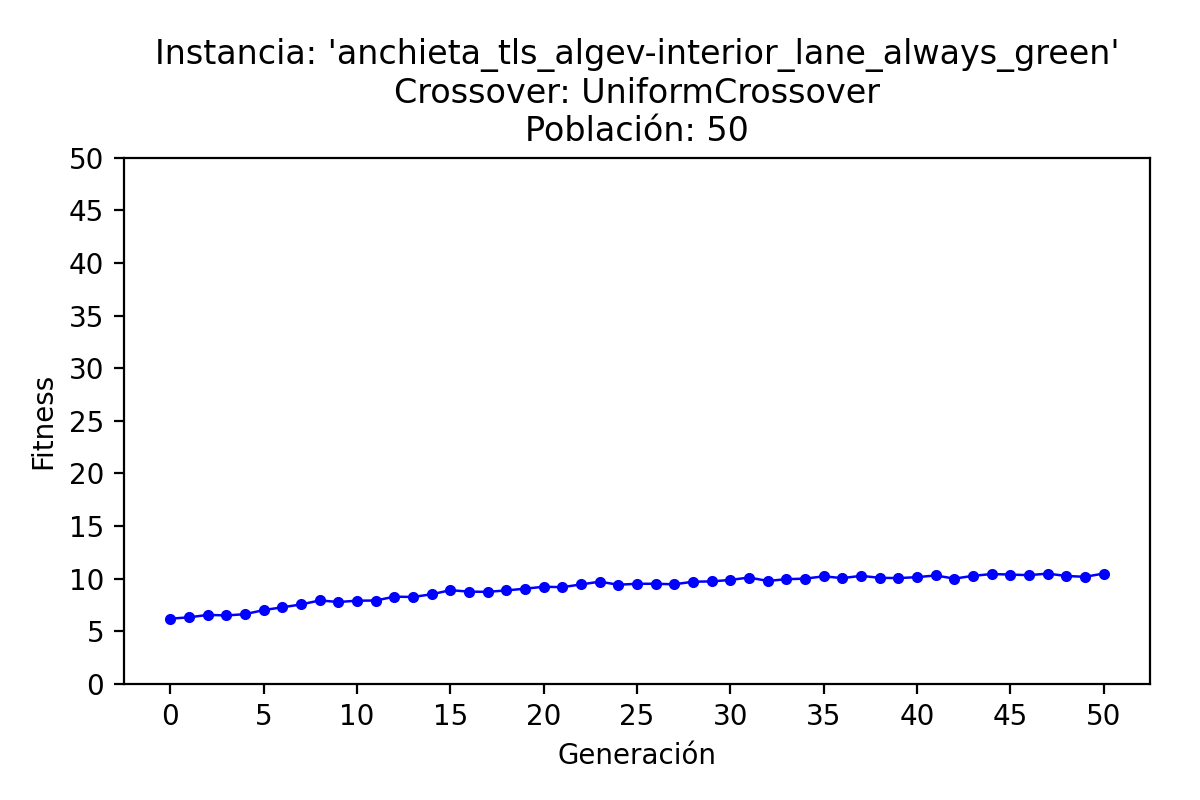
\includegraphics[width=\textwidth]{report/images/estudio/anchieta_tls_algev-interior_lane_always_green-UniformCrossover-50.png}
    \end{subfigure}
    \caption{Evolución del fitness medio entre ejecuciones del mejor candidato de cada generación para la instancia S\textsubscript{4}}
    \label{fig:estudio:anchieta_tls_interior_lane_always_green}
\end{figure}

\subsection{Instancia S\textsubscript{5}: <<anchieta\_tls\_interior\_lane\_changes>>}

Lo cierto es que el estudio de esta instancia arroja resultados similares a los de la instancia anterior. El estudio de la evolución del fitess, que puede apreciarse en la Figura~\ref{fig:estudio:anchieta_tls_interior_lane_changes}, parece resaltar que, al igual que con la instancia anterior, el fitness mejora al usar una población mayor. Sin embargo, esta instancia proporciona, de manera general, un valor de fitness más alto que la anterior; y en el caso de las comparativas entre cruces, la diferencia en el valor del fitness es más acusada.

Observando los resultados de la evaluación por parejas de las diferentes configuraciones de la Tabla~\ref{tab:estudio:anchieta_tls_interior_lane_changes}, los resultados quedan idénticos a los de la instancia anterior, terminando como ganador el conjunto de parámetros que emplea el cruce \texttt{UniformCrossover} y una población de 50 individuos. En segundo lugar, queda el conjunto \texttt{OnePointCrossover} y población 50 individuos; y de la misma manera, se comprueba que no hay diferencia en emplear uno u otro cruce cuando la población es de 10 invididuos.

\begin{figure}[h]
    \centering
    \begin{subfigure}[t]{.49\textwidth}
      \centering
      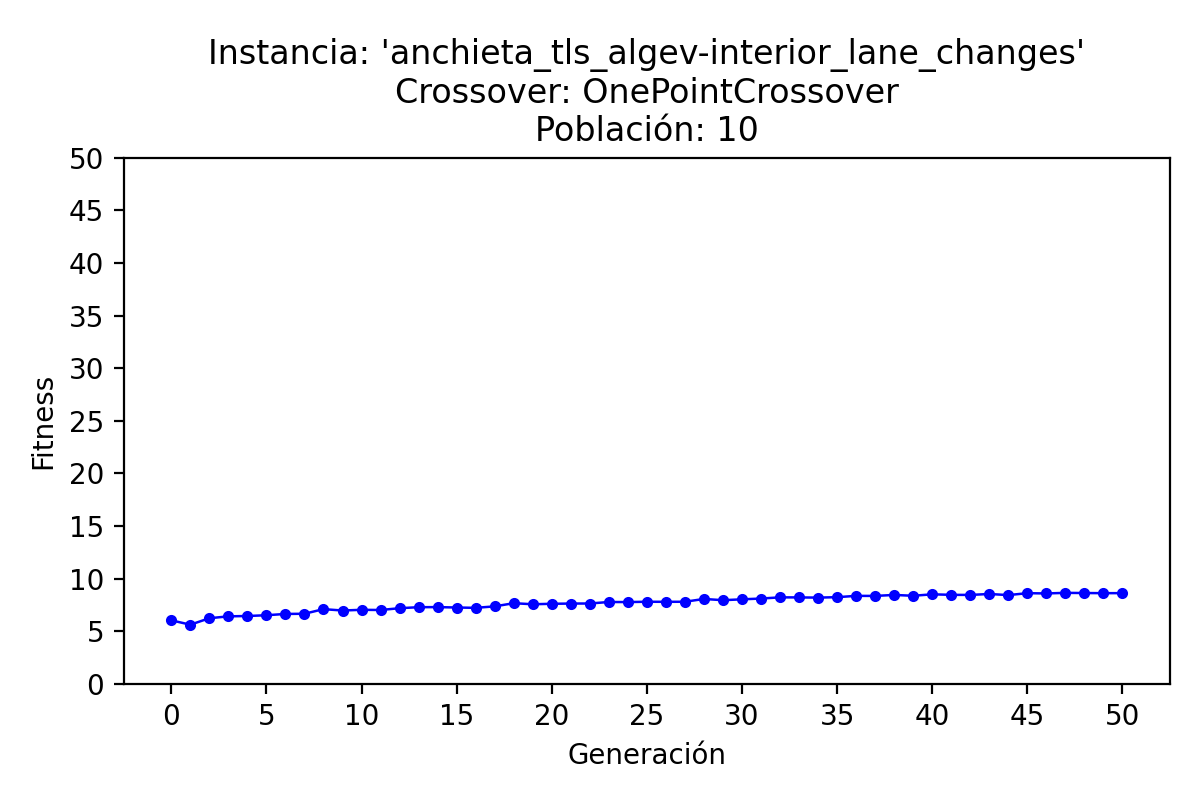
\includegraphics[width=\textwidth]{report/images/estudio/anchieta_tls_algev-interior_lane_changes-OnePointCrossover-10.png}
    \end{subfigure}
    \hfill
    \begin{subfigure}[t]{.49\textwidth}
      \centering
      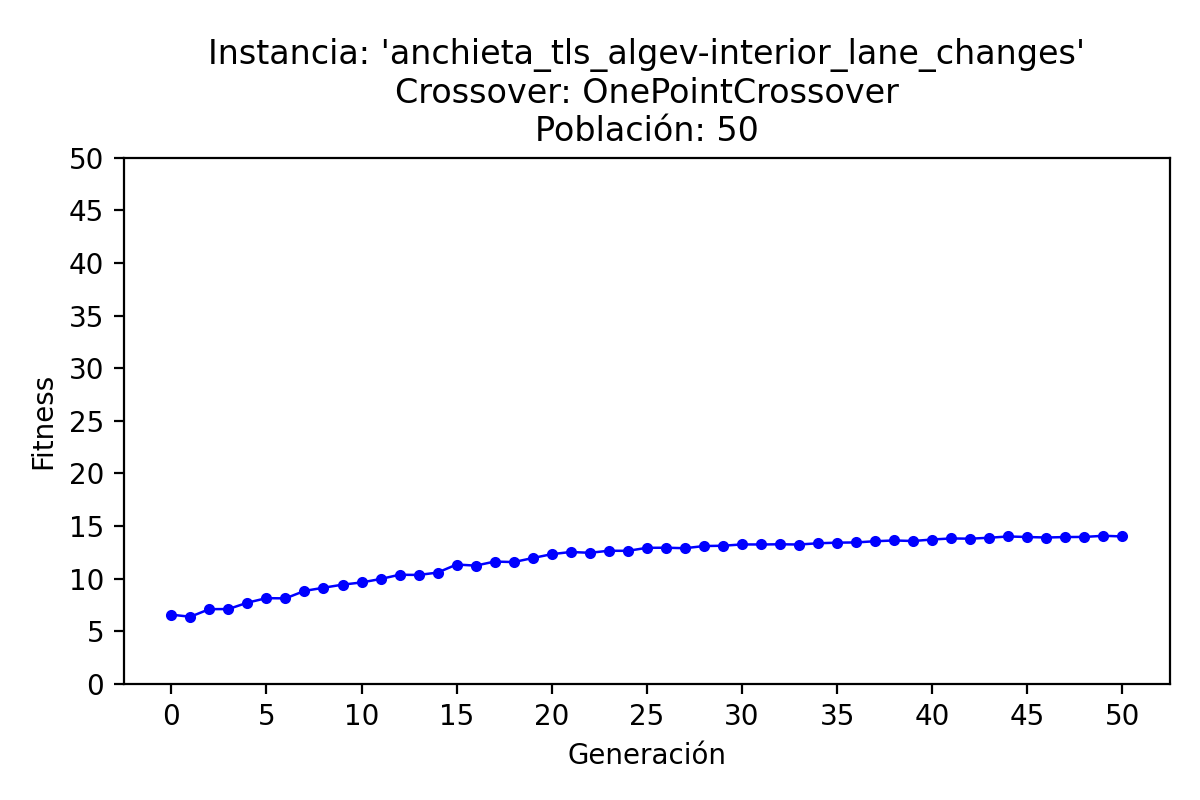
\includegraphics[width=\textwidth]{report/images/estudio/anchieta_tls_algev-interior_lane_changes-OnePointCrossover-50.png}
    \end{subfigure}
    \vspace{0.7cm}
    \begin{subfigure}[t]{.49\textwidth}
      \centering
      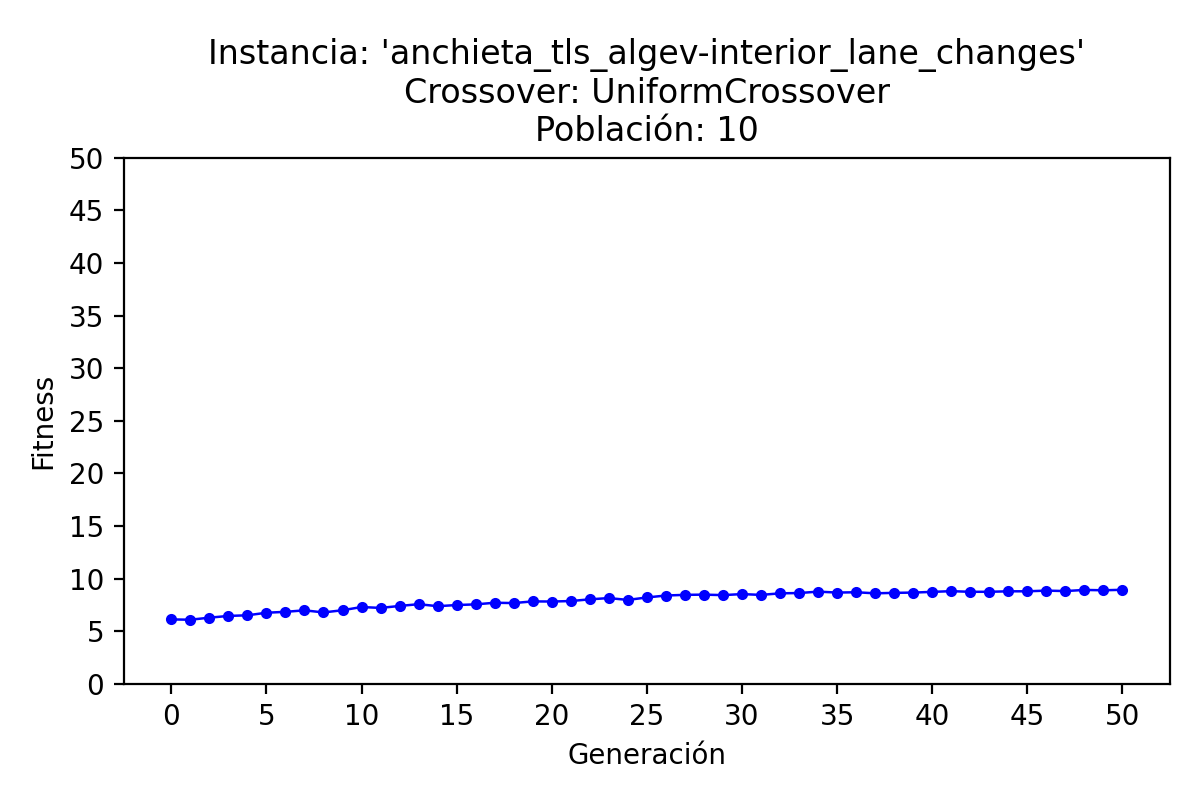
\includegraphics[width=\textwidth]{report/images/estudio/anchieta_tls_algev-interior_lane_changes-UniformCrossover-10.png}
    \end{subfigure}
    \hfill
    \begin{subfigure}[t]{.49\textwidth}
      \centering
      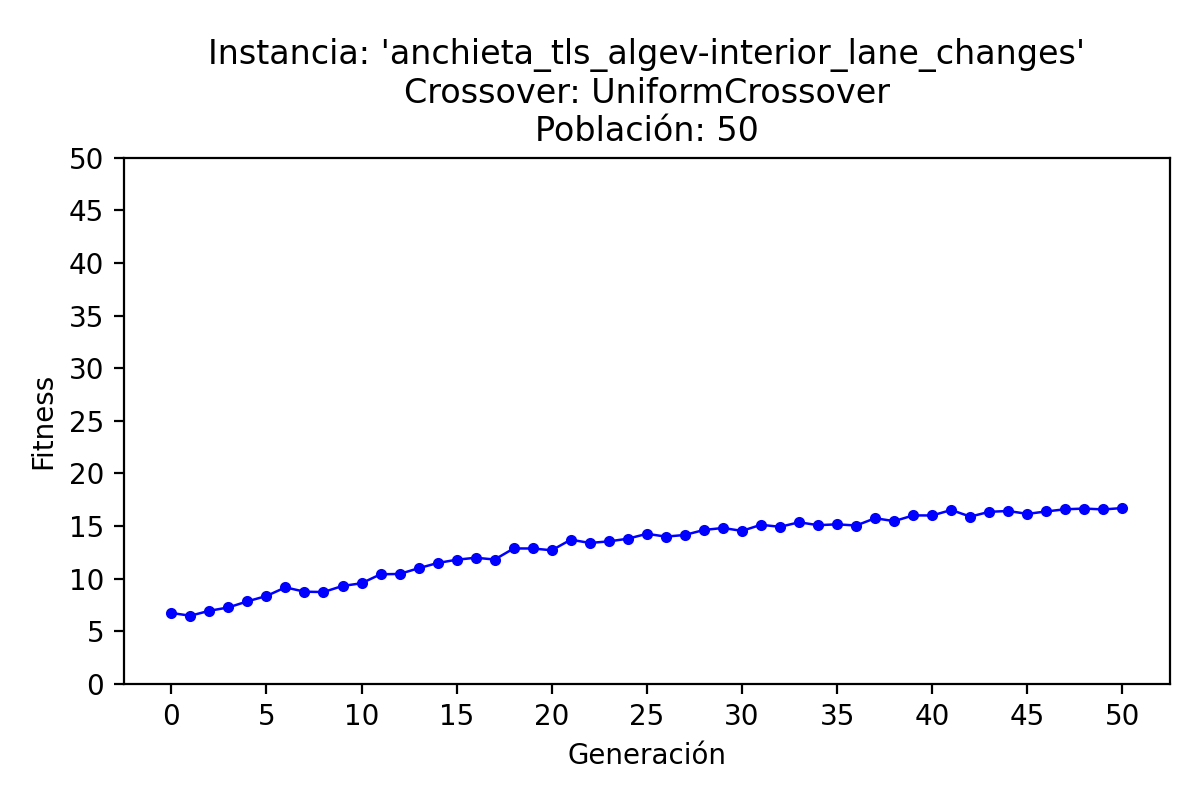
\includegraphics[width=\textwidth]{report/images/estudio/anchieta_tls_algev-interior_lane_changes-UniformCrossover-50.png}
    \end{subfigure}
    \caption{Evolución del fitness medio entre ejecuciones del mejor candidato de cada generación para la instancia S\textsubscript{5}}
    \label{fig:estudio:anchieta_tls_interior_lane_changes}
\end{figure}



\subsection{Instancia S\textsubscript{6}: <<anchieta\_tls\_few\_pedestrians>>}

En comparación con las anteriores, los resultados de la evaluación del fitness de esta instancia (Figura~\ref{fig:estudio:anchieta_tls_special_few_pedestrians}) arrojan resultados mucho mayores; por lo cual se aprecia que la utilización de menos semáforos redunda en un incremento bastante acusado del fitness. Asímismo, y en consonancia con las evaluaciones anteriores, la diferencia en la población se cristaliza una vez más como causante de un incremento en el fitness en el caso de ambos cruces, dando mejores resultados la utilización 50 individuos por generación.

Sin embargo, observando los resultados de la evaluación de los conjuntos de parámetros (Tabla~\ref{tab:estudio:anchieta_tls_special_few_pedestrians}), se puede apreciar como los conjuntos \texttt{OnePointCrossover/Pob50} y \texttt{UniformCrossover/Pob50} llegan a un empate en el cual ambos han ganado (y perdido) la misma cantidad de veces en las evaluaciones con otros conjuntos, además de que no se aprecia diferencia estadística entre uno y otro. Así pues, la conclusión es que realmente no hay diferencia entre emplear cualquiera de los dos, puesto que brindaran resultados extremadamente parecidos.

\begin{figure}[h]
    \centering
    \begin{subfigure}[t]{.49\textwidth}
      \centering
      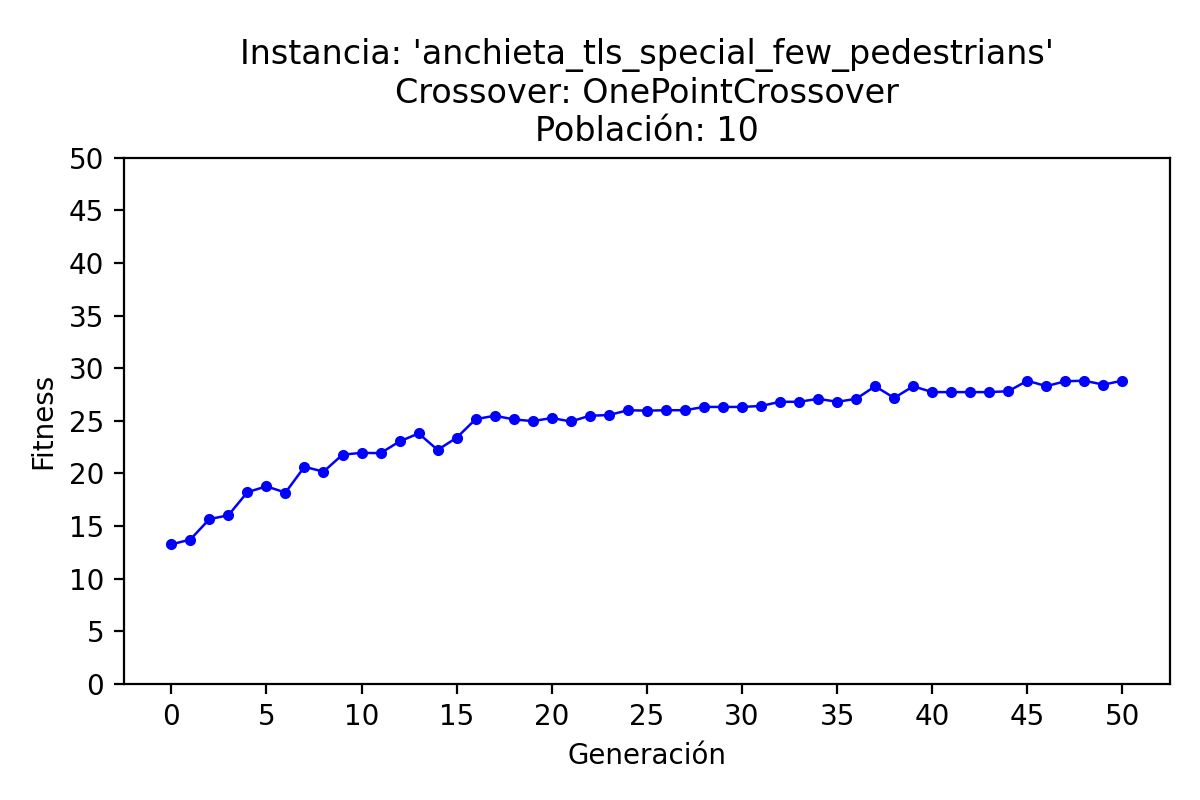
\includegraphics[width=\textwidth]{report/images/estudio/anchieta_tls_special_few_pedestrians-OnePointCrossover-10.png}
    \end{subfigure}
    \hfill
    \begin{subfigure}[t]{.49\textwidth}
      \centering
      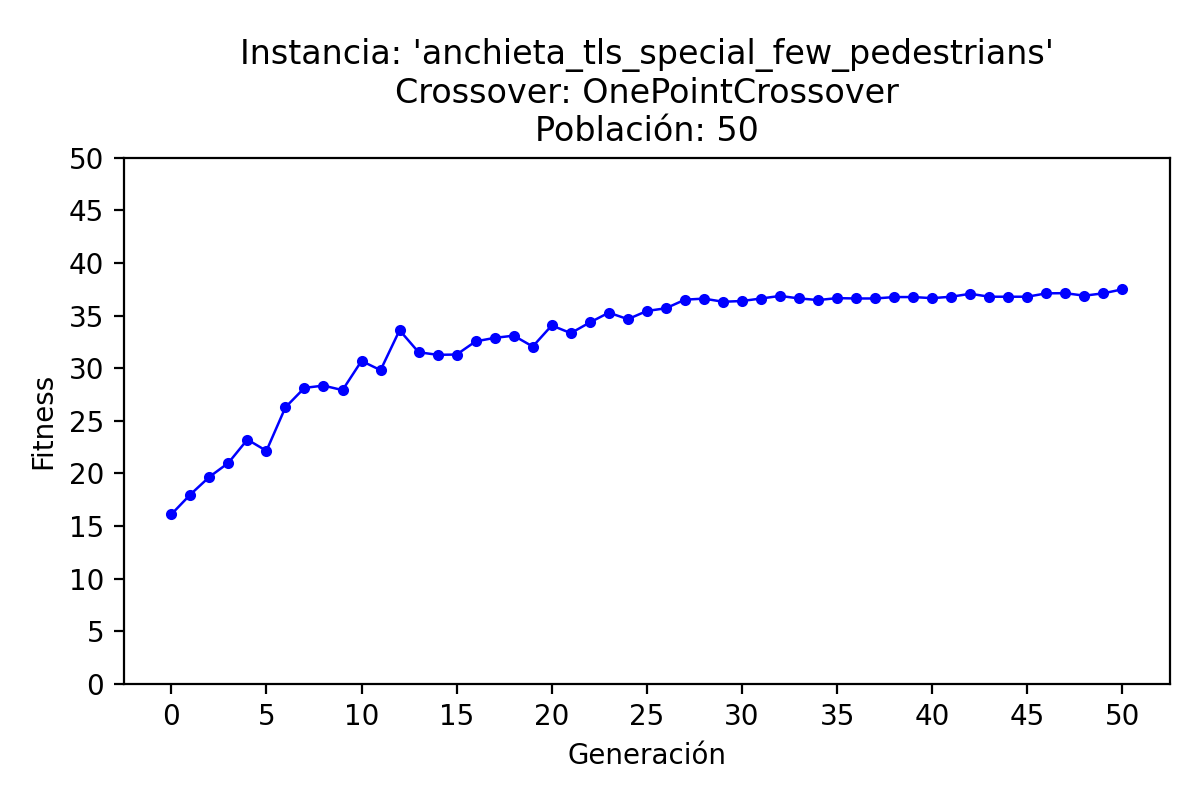
\includegraphics[width=\textwidth]{report/images/estudio/anchieta_tls_special_few_pedestrians-OnePointCrossover-50.png}
    \end{subfigure}
    \vspace{0.7cm}
    \begin{subfigure}[t]{.49\textwidth}
      \centering
      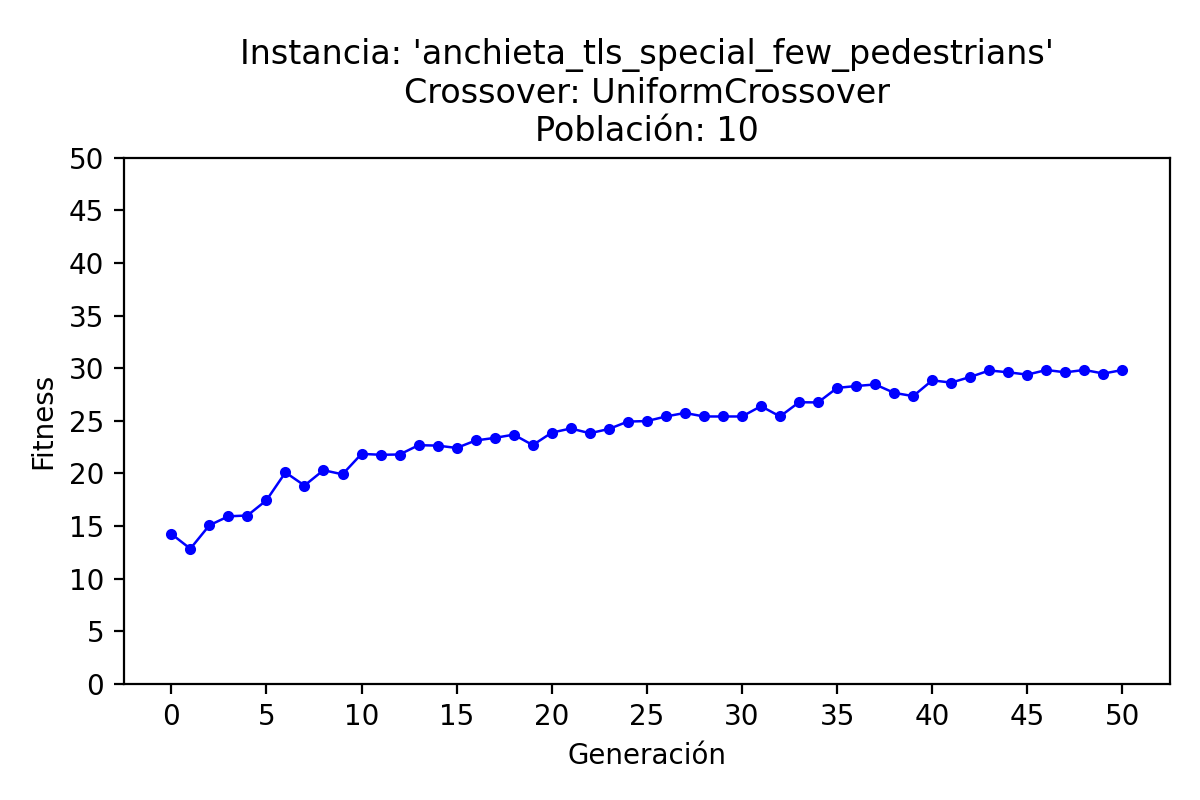
\includegraphics[width=\textwidth]{report/images/estudio/anchieta_tls_special_few_pedestrians-UniformCrossover-10.png}
    \end{subfigure}
    \hfill
    \begin{subfigure}[t]{.49\textwidth}
      \centering
      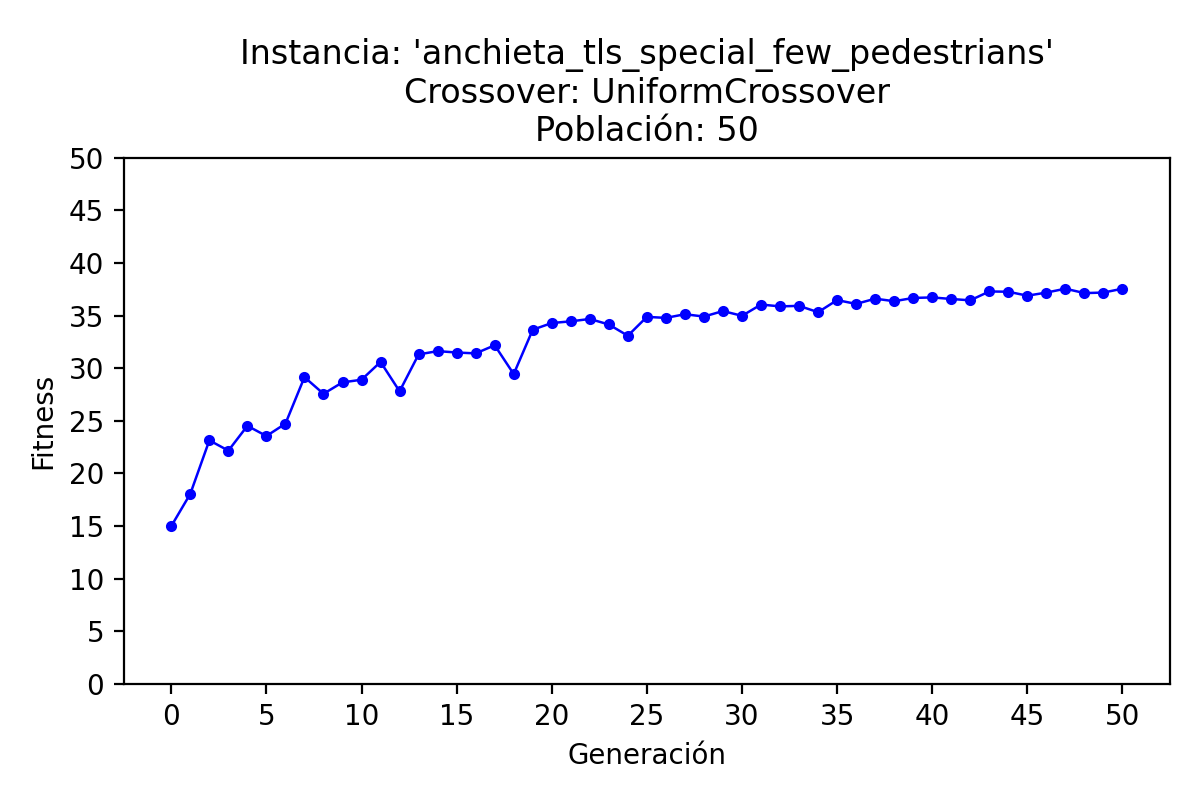
\includegraphics[width=\textwidth]{report/images/estudio/anchieta_tls_special_few_pedestrians-UniformCrossover-50.png}
    \end{subfigure}
    \caption{Evolución del fitness medio entre ejecuciones del mejor candidato de cada generación para la instancia S\textsubscript{6}}
    \label{fig:estudio:anchieta_tls_special_few_pedestrians}
\end{figure}



\subsection{Instancia S\textsubscript{7}: <<anchieta\_tls\_many\_pedestrians>>}

La evaluación del fitness de cada conjunto de parámetros empleado en esta instancia ofrece resultados interesantes si se compara con la anterior, puesto que es fácil apreciar una reducción considerable del fitness en todos los casos, tal y como se puede apreciar en la Figura~\ref{fig:estudio:anchieta_tls_special_many_pedestrians}.  

Observando los resultados de la competición entre sí de cada conjunto (Tabla~\ref{tab:estudio:anchieta_tls_special_many_pedestrians}), se comprueba que los resultados son idénticos a los de la instancia anterior, con un empate entre los conjuntos \texttt{OnePointCrossover/Pob50} y \texttt{UniformCrossover/Pob50}; de modo que no hay diferencia entre emplear uno u otro.

\begin{figure}[h]
    \centering
    \begin{subfigure}[t]{.49\textwidth}
      \centering
      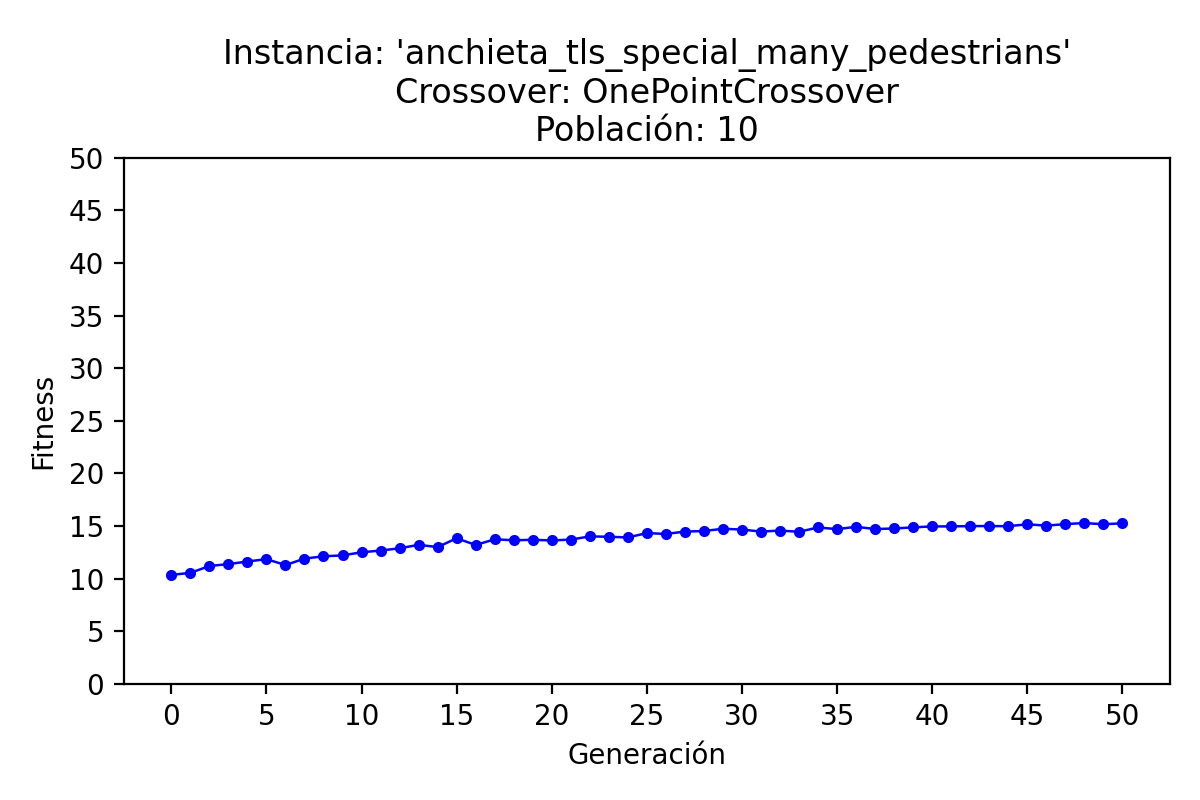
\includegraphics[width=\textwidth]{report/images/estudio/anchieta_tls_special_many_pedestrians-OnePointCrossover-10.png}
    \end{subfigure}
    \hfill
    \begin{subfigure}[t]{.49\textwidth}
      \centering
      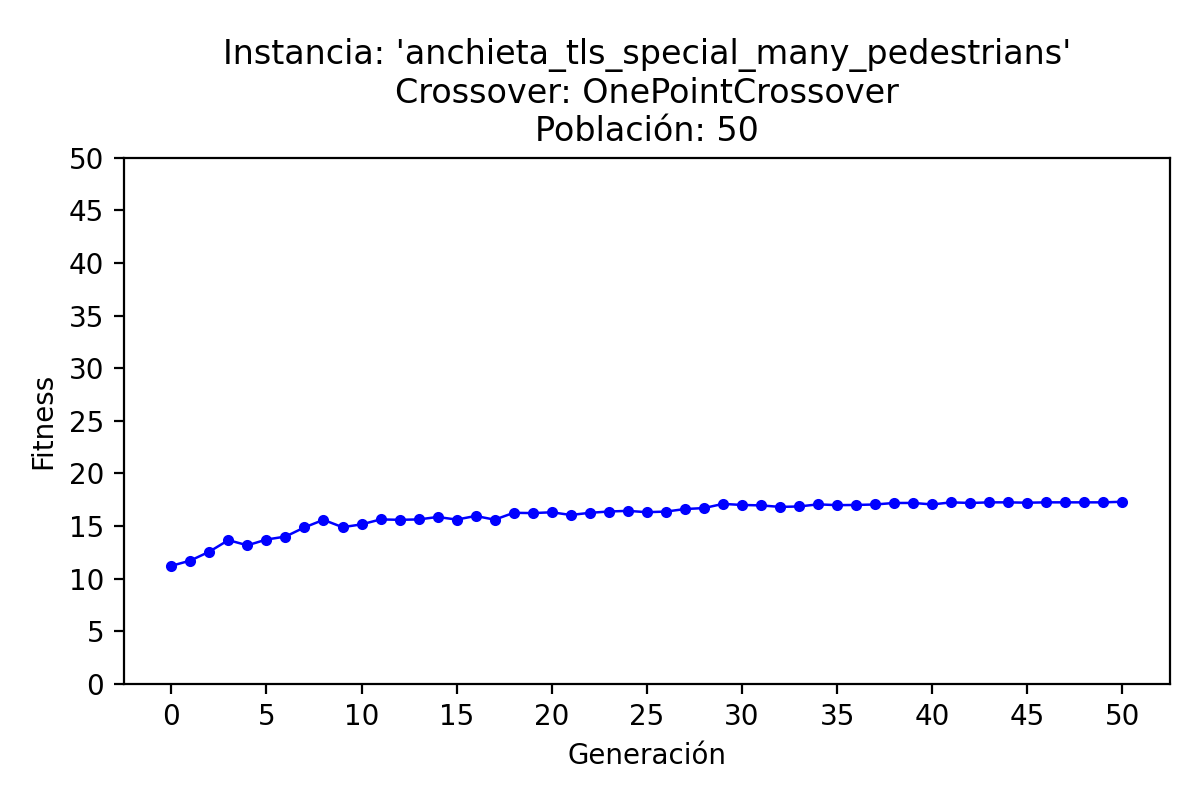
\includegraphics[width=\textwidth]{report/images/estudio/anchieta_tls_special_many_pedestrians-OnePointCrossover-50.png}
    \end{subfigure}
    \vspace{0.7cm}
    \begin{subfigure}[t]{.49\textwidth}
      \centering
      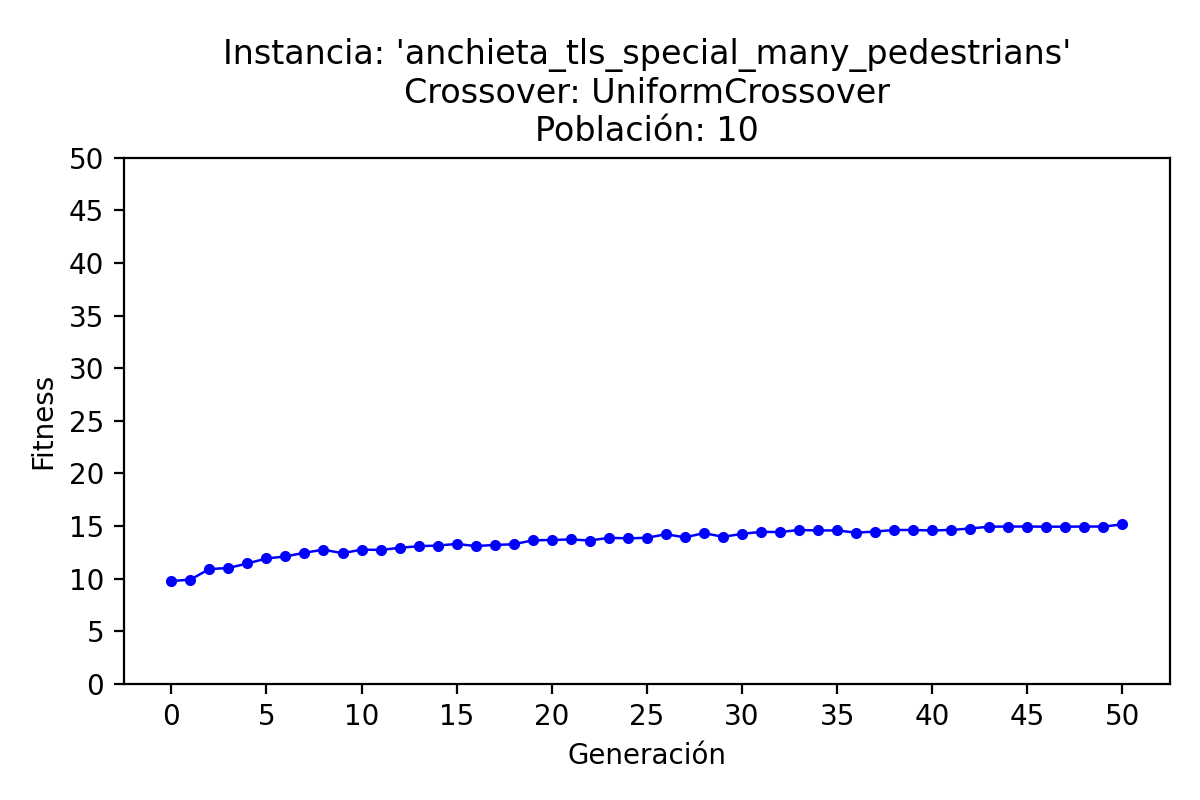
\includegraphics[width=\textwidth]{report/images/estudio/anchieta_tls_special_many_pedestrians-UniformCrossover-10.png}
    \end{subfigure}
    \hfill
    \begin{subfigure}[t]{.49\textwidth}
      \centering
      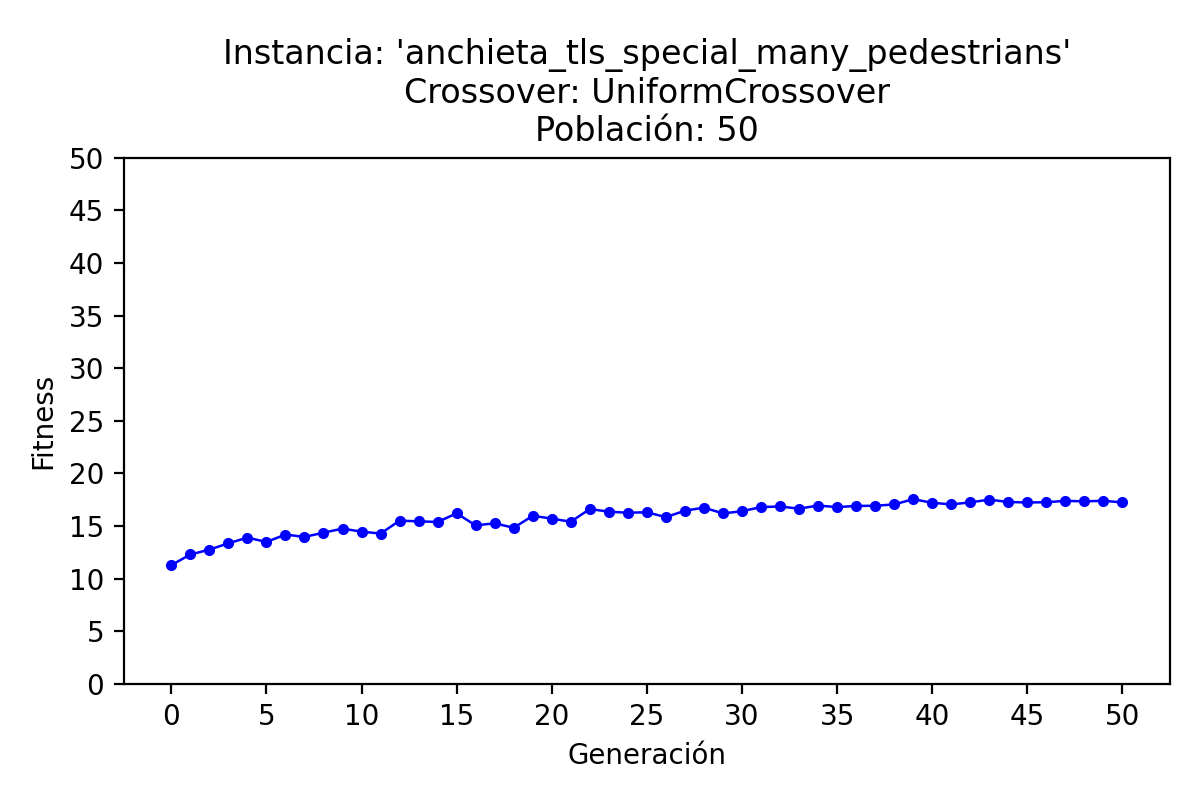
\includegraphics[width=\textwidth]{report/images/estudio/anchieta_tls_special_many_pedestrians-UniformCrossover-50.png}
    \end{subfigure}
    \caption{Evolución del fitness medio entre ejecuciones del mejor candidato de cada generación para la instancia S\textsubscript{7}}
    \label{fig:estudio:anchieta_tls_special_many_pedestrians}
\end{figure}


\subsection{Análisis de los resultados}

Realizada una evaluación de las configuraciones anteriores, para la simulación se emplearán las instancias obtenidas del algoritmo evolutivo con los siguientes conjuntos de parámetros:

\begin{itemize}
    \item \textbf{anchieta\_tls\_interior\_lane\_always\_green:}: \texttt{UniformCrossover/Pob50}
    \item \textbf{anchieta\_tls\_interior\_lane\_changes:} \texttt{UniformCrossover/Pob50}
    \item \textbf{anchieta\_tls\_few\_pedestrians:} \texttt{UniformCrossover/Pob50}
    \item \textbf{anchieta\_tls\_many\_pedestrians:} \texttt{UniformCrossover/Pob50}
\end{itemize}



% TABLAS

\begin{sidewaystable}[h]
    \bigskip\bigskip
    \caption{}
    \label{tab:estudio:anchieta_tls_special_few_pedestrians}
    \resizebox{\textwidth}{!}{\begin{tabular}{lllllll}
    \hline
    \multicolumn{7}{c}{\textbf{anchieta\_tls\_few\_pedestrians}}                                                                                                                                                                                             \\ \hline
    \multicolumn{1}{c}{\multirow{2}{*}{\textit{Conjuntos de parámetros 1 y 2}}}        & \multicolumn{2}{c}{\textit{Media}}            & \multicolumn{2}{c}{\textit{Mediana}}          & \multicolumn{1}{c}{\multirow{2}{*}{\textit{p-value}}} & \multicolumn{1}{c}{\multirow{2}{*}{\textit{Ganador}}} \\ \cline{2-5}
    \multicolumn{1}{c}{}                                                & \multicolumn{1}{c}{1} & \multicolumn{1}{c}{2} & \multicolumn{1}{c}{1} & \multicolumn{1}{c}{2} & \multicolumn{1}{c}{}                                  & \multicolumn{1}{c}{}                                  \\ \hline
    OnePointCrossover/Pop10 y OnePointCrossover/Pop50                   & 29.45247              & 37.67554              & 27.4298               & 38.05608              & 0.0002177574                                          & OnePointCrossover/Pop50                               \\ \hline
    OnePointCrossover/Pop10 y UniformCrossover/Pop10                    & 29.45247              & 29.88526              & 27.4298               & 28.53967              & 0.8623907                                             & No hay diferencia estadística                         \\ \hline
    OnePointCrossover/Pop10 y UniformCrossover/Pop50                    & 29.45247              & 38.31307              & 27.4298               & 38.35384              & 0.0003900244                                          & UniformCrossover/Pop50                                \\ \hline
    OnePointCrossover/Pop50 y UniformCrossover/Pop10                    & 37.67554              & 29.88526              & 38.05608              & 28.53967              & 0.00180757                                            & OnePointCrossover/Pop50                               \\ \hline
    OnePointCrossover/Pop50 y UniformCrossover/Pop50                    & 37.67554              & 38.31307              & 38.05608              & 38.35384              & 0.4469909                                             & No hay diferencia estadística                         \\ \hline
    UniformCrossover/Pop10 y UniformCrossover/Pop50                     & 29.88526              & 38.31307              & 28.53967              & 38.35384              & 0.001050841                                           & UniformCrossover/Pop50                                \\ \hline
    \end{tabular}}
    
    \bigskip\bigskip
    \caption{}
    \label{tab:estudio:anchieta_tls_special_many_pedestrians}
    \resizebox{\textwidth}{!}{\begin{tabular}{lllllll}
    \hline
    \multicolumn{7}{c}{\textbf{anchieta\_tls\_many\_pedestrians}}                                                                                                                                                                                            \\ \hline
    \multicolumn{1}{c}{\multirow{2}{*}{\textit{Conjuntos de parámetros 1 y 2}}}        & \multicolumn{2}{c}{\textit{Media}}            & \multicolumn{2}{c}{\textit{Mediana}}          & \multicolumn{1}{c}{\multirow{2}{*}{\textit{p-value}}} & \multicolumn{1}{c}{\multirow{2}{*}{\textit{Ganador}}} \\ \cline{2-5}
    \multicolumn{1}{c}{}                                                & \multicolumn{1}{c}{1} & \multicolumn{1}{c}{2} & \multicolumn{1}{c}{1} & \multicolumn{1}{c}{2} & \multicolumn{1}{c}{}                                  & \multicolumn{1}{c}{}                                  \\ \hline
    OnePointCrossover/Pop10 y OnePointCrossover/Pop50                   & 15.3666               & 17.38808              & 15.65755              & 17.53609              & 7.402106e-05                                          & OnePointCrossover/Pop50                               \\ \hline
    OnePointCrossover/Pop10 y UniformCrossover/Pop10                    & 15.3666               & 15.26587              & 15.65755              & 15.11698              & 0.86804                                               & No hay diferencia estadística                         \\ \hline
    OnePointCrossover/Pop10 y UniformCrossover/Pop50                    & 15.3666               & 17.72223              & 15.65755              & 17.9043               & 4.202438e-05                                          & UniformCrossover/Pop50                                \\ \hline
    OnePointCrossover/Pop50 y UniformCrossover/Pop10                    & 17.38808              & 15.26587              & 17.53609              & 15.11698              & 0.001255819                                           & OnePointCrossover/Pop50                               \\ \hline
    OnePointCrossover/Pop50 y UniformCrossover/Pop50                    & 17.38808              & 17.72223              & 17.53609              & 17.9043               & 0.390172                                              & No hay diferencia estadística                         \\ \hline
    UniformCrossover/Pop10 y UniformCrossover/Pop50                     & 15.26587              & 17.72223              & 15.11698              & 17.9043               & 0.0005555893                                          & UniformCrossover/Pop50                                \\ \hline
    \end{tabular}}
\end{sidewaystable}


\begin{sidewaystable}
    \caption{Resultado de la comparación por parejas de la instancia anchieta\_tls\_interior\_lane\_always\_green}
    \label{tab:estudio:anchieta_tls_interior_lane_always_green}
    \resizebox{\textwidth}{!}{\begin{tabular}{lllllll}
    \hline
    \multicolumn{7}{c}{\textbf{anchieta\_tls\_interior\_lane\_always\_green}}                                                                                                                                                                                   \\ \hline
    \multicolumn{1}{c}{\multirow{2}{*}{\textit{Conjuntos de parámetros 1 y 2}}}        & \multicolumn{2}{c}{\textit{Media}}            & \multicolumn{2}{c}{\textit{Mediana}}          & \multicolumn{1}{c}{\multirow{2}{*}{\textit{p-value}}} & \multicolumn{1}{c}{\multirow{2}{*}{\textit{Ganador}}} \\ \cline{2-5}
    \multicolumn{1}{c}{}                                                & \multicolumn{1}{c}{1} & \multicolumn{1}{c}{2} & \multicolumn{1}{c}{1} & \multicolumn{1}{c}{2} & \multicolumn{1}{c}{}                                  & \multicolumn{1}{c}{}                                  \\ \hline
    OnePointCrossover/Pop10 y OnePointCrossover/Pop50                   & 7.364113              & 9.962546              & 7.298901              & 10.05993              & 5.78933e-05                                           & OnePointCrossover/Pop50                               \\ \hline
    OnePointCrossover/Pop10 y UniformCrossover/Pop10                    & 7.364113              & 7.859806              & 7.298901              & 7.632471              & 0.1928009                                             & No hay diferencia estadística                         \\ \hline
    OnePointCrossover/Pop10 y UniformCrossover/Pop50                    & 7.364113              & 11.16813              & 7.298901              & 11.15414              & 0.0001570523                                          & UniformCrossover/Pop50                                \\ \hline
    OnePointCrossover/Pop50 y UniformCrossover/Pop10                    & 9.962546              & 7.859806              & 10.05993              & 7.632471              & 0.0001639967                                          & OnePointCrossover/Pop50                               \\ \hline
    OnePointCrossover/Pop50 y UniformCrossover/Pop50                    & 9.962546              & 11.16813              & 10.05993              & 11.15414              & 0.0101652                                             & UniformCrossover/Pop50                                \\ \hline
    UniformCrossover/Pop10 y UniformCrossover/Pop50                     & 7.859806              & 11.16813              & 7.632471              & 11.15414              & 0.0001570523                                          & UniformCrossover/Pop50                                \\ \hline
    \end{tabular}}
    
    
    
    \bigskip\bigskip
    \caption{Resultado de la comparación por parejas de la instancia anchieta\_tls\_interior\_lane\_changes}
    \label{tab:estudio:anchieta_tls_interior_lane_changes}
    \resizebox{\textwidth}{!}{\begin{tabular}{lllllll}
    \hline
    \multicolumn{7}{c}{\textbf{anchieta\_tls\_interior\_lane\_changes}}                                                                                                                                                                                         \\ \hline
    \multicolumn{1}{c}{\multirow{2}{*}{\textit{Conjuntos de parámetros 1 y 2}}}        & \multicolumn{2}{c}{\textit{Media}}            & \multicolumn{2}{c}{\textit{Mediana}}          & \multicolumn{1}{c}{\multirow{2}{*}{\textit{p-value}}} & \multicolumn{1}{c}{\multirow{2}{*}{\textit{Ganador}}} \\ \cline{2-5}
    \multicolumn{1}{c}{}                                                & \multicolumn{1}{c}{1} & \multicolumn{1}{c}{2} & \multicolumn{1}{c}{1} & \multicolumn{1}{c}{2} & \multicolumn{1}{c}{}                                  & \multicolumn{1}{c}{}                                  \\ \hline
    OnePointCrossover/Pop10 y OnePointCrossover/Pop50                   & 8.654163              & 14.24831              & 8.53437               & 14.10958              & 1.21893e-06                                           & OnePointCrossover/Pop50                               \\ \hline
    OnePointCrossover/Pop10 y UniformCrossover/Pop10                    & 8.654163              & 9.004224              & 8.53437               & 8.693441              & 0.6450571                                             & No hay diferencia estadística                         \\ \hline
    OnePointCrossover/Pop10 y UniformCrossover/Pop50                    & 8.654163              & 17.58131              & 8.53437               & 17.49452              & 1.79459e-09                                           & UniformCrossover/Pop50                                \\ \hline
    OnePointCrossover/Pop50 y UniformCrossover/Pop10                    & 14.24831              & 9.004224              & 14.10958              & 8.693441              & 2.836182e-06                                          & OnePointCrossover/Pop50                               \\ \hline
    OnePointCrossover/Pop50 y UniformCrossover/Pop50                    & 14.24831              & 17.58131              & 14.10958              & 17.49452              & 0.000899443                                           & UniformCrossover/Pop50                                \\ \hline
    UniformCrossover/Pop10 y UniformCrossover/Pop50                     & 9.004224              & 17.58131              & 8.693441              & 17.49452              & 3.310727e-09                                          & UniformCrossover/Pop50                                \\ \hline
    \end{tabular}}
\end{sidewaystable}




\section{Simulación}

Una vez hemos evaluado cual de las configuraciones 

\begin{sidewaystable}
    \caption{Resultados de la ejecución de la simulación empleando la configuración óptima}
    \label{tab:estudio:resultados}
    \resizebox{\textwidth}{!}{\begin{tabular}{llllllllllllll}
    \hline
    \multicolumn{14}{c}{\textbf{Resultados de la simulación}}                                                                                                                                                                                                                                                                                                                                                                                                     \\ \hline
    \multicolumn{1}{c}{\multirow{2}{*}{\textit{Instancia}}} & \multicolumn{4}{c}{\textit{Vehículos}}                                                                                             &  & \multicolumn{6}{c}{\textit{Estadísticas}}                                                                                                                                                                            &  & \multirow{2}{*}{\textit{Fitness}} \\ \cline{2-5} \cline{7-12}
    \multicolumn{1}{c}{}                                    & \multicolumn{1}{c}{Cargados} & \multicolumn{1}{c}{Insertados} & \multicolumn{1}{c}{En ejecución} & \multicolumn{1}{c}{A la espera} &  & \multicolumn{1}{c}{Longitud (m)} & \multicolumn{1}{c}{Velocidad (m/s)} & \multicolumn{1}{c}{T. perdido (s)} & \multicolumn{1}{c}{T. espera (s)} & \multicolumn{1}{c}{Duración (s)} & \multicolumn{1}{c}{Retardo (s)} &  &                                   \\ \hline
    anchieta\_no\_tls                                       & 14181.8                      & 13057.8                        & 614.6                            & 1124                            &  & 1705.982                         & 22.99                               & 88.34                              & 145.44                            & 44.94                            & 70.55                           &  & 21.71                             \\ \hline
    anchieta\_no\_tls\_few\_pedestrians                     & 14182.8                      & 12904.8                        & 623.4                            & 1278                            &  & 1713.93                          & 23.253                              & 91.304                             & 148.404                           & 50.476                           & 71.458                          &  & 18.85                             \\ \hline
    anchieta\_no\_tls\_many\_pedestrians                    & 14182.7                      & 12878.1                        & 640.1                            & 1304.6                          &  & 1707.695                         & 23.125                              & 94.263                             & 151.237                           & 51.693                           & 80.753                          &  & 17.41                             \\ \hline
    anchieta\_tls\_interior\_lane\_always\_green      & 14184                        & 11954.1                        & 761.8                            & 2229.9                          &  & 1739.027                         & 23.883                              & 145.692                            & 201.943                           & 110.81                           & 85.724                          &  & 7.50                              \\ \hline
    anchieta\_tls\_interior\_lane\_changes            & 14183.6                      & 12397.3                        & 781                              & 1786.3                          &  & 1708.098                         & 23.332                              & 130.275                            & 186.185                           & 91.921                           & 95.318                          &  & 10.59                             \\ \hline
    anchieta\_tls\_few\_pedestrians                & 14181.7                      & 12669.1                        & 678.4                            & 1512.6                          &  & 1726.209                         & 23.32                               & 106.309                            & 163.292                           & 61.791                           & 87.167                          &  & 15.01                             \\ \hline
    anchieta\_tls\_many\_pedestrians               & 14183.1                      & 12699.2                        & 737                              & 1483.9                          &  & 1763.325                         & 23.436                              & 115.69                             & 173.26                            & 71.151                           & 59.275                          &  & 14.09                             \\ \hline
    \end{tabular}}
\end{sidewaystable}


\subsection{Análisis de los resultados}
\chapter{Conclusiones y líneas futuras}
\label{cap:conclusiones}

El objetivo de este Trabajo de Fin de Grado residía en averiguar si, con la instalación de semáforos optimizados por un algoritmo evolutivo, era posible mejorar el tráfico de la rotonda del Padre Anchieta, evitando así la ralentización del tráfico que día tras día se produce en horas punta debido a la gran afluencia de vehículos y peatones que circulan a través de la rotonda. Para llevar a cabo el proyecto, se empleó SUMO como simulador de tráfico, y Genetics.js para la ejecución del algoritmo evolutivo. El problema a resolver no es otro que el TLSP \textit{(Traffic Light Scheduling Problem)}: la optimización de la duración de las fases de los semáforos; en este caso, empleando un algoritmo genético.

Para ello, se han obtenido un mapa de la zona de la rotonda del Padre Anchieta gracias a OpenStreetMap. Posteriormente, dicho mapa se convirtió al formato de un archivo de red legible por el simulador (gracias a \texttt{NETCONVERT}) y ha sido modificado profusamente para: incorporar semáforos, pasos de peatones, aceras, corregir la forma y algunos datos de las vías (por ejemplo: la velocidad, la cual era incorrecta en algunas vías), la forma de las intersecciones, etc. Todo ello fue realizado con \texttt{NETEDIT}, un programa de manipulación de archivos de red. Esto nos ha brindado un archivo que representa con un alto nivel de fiabilidad las vías de la zona de la rotonda. 

Asimismo, se ha generado un archivo de tráfico en función de datos de aforadores obtenidos por el Cabildo de Tenerife, en un estudio realizado por la corporación en noviembre de 2019. El archivo de tráfico ha sido generado a partir del tratamiento de los datos de los aforadores, con una herramienta del simulador (\texttt{flowrouter.py}) que permite generar flujos de tráfico sobre el archivo de red a partir de estos datos. Finalmente, los peatones se han generado de manera aleatoria y uniforme debido a que no existe información sobre la circulación de peatones en la zona.

A continuación, se diseñaron un conjunto de instancias en función de la configuración de los semáforos y de la cantidad de peatones que circularían por la zona. En total, fueron siete: tres instancias sin semáforos, y cuatro con semáforos. La principal diferencia en las instancias sin semáforos era la cantidad de peatones, que iba desde ninguno hasta \textasciitilde2000. Respecto a las instancias con semáforos, se pueden dividir en dos grupos. El primero incluía semáforos en todas las entradas y salidas, variando el comportamiento del carril interno de la rotonda, de modo que en una instancia los semáforos de este carril estaban siempre en verde (cuando la intersección lo permitía), mientras que en la otra los semáforos variaban junto con los del carril exterior. El segundo grupo de instancias solo incluía semáforos al norte y al sur de la rotonda, variando únicamente en la cantidad de peatones.

Diseñadas las instancias, se llevó a cabo un estudio estadístico previo para determinar cuáles de los parámetros del algoritmo genético eran los indicados para cada instancia (únicamente de las que tienen semáforos), de modo que se pudieran obtener mejores resultados con la ejecución del algoritmo. Dicho estudio se centró en evaluar dos parámetros distintos: el tipo de cruce empleado (\texttt{UniformCrossover} o \texttt{OnePointCrossover}) y el tamaño de la población (10 o 50). Realizado el estudio de todas las configuraciones posibles para cada una instancia, se compararon en parejas y se realizó una clasificación para determinar cual de las configuraciones obtenía mejores resultados. La conclusión alcanzada fue que el cruce \texttt{UniformCrossover} y una población con 50 individuos proporcionaba los mejores resultados en general para dos de las cuatro instancias, mientras que para las otras dos no había diferencia entre emplear dicha configuración y \texttt{OnePointCrossover} y una población de tamaño 50. Así pues, se empleó la primera por simple comodidad para realizar la simulación final.

Finalmente, evaluando los resultados provistos por SUMO para cada instancia, se pudo apreciar que ninguna de ellas ofrece un tráfico más eficiente que la instancia sin peatones ni semáforos. Por otro lado, ninguna de las instancias con semáforos consiguió mejorar los resultados de la instancia sin semáforos con mayor cantidad de peatones, lo que indica que el empleo de semáforos en la rotonda no mejorará el tráfico, aún cuando sus fases han sido optimizadas.

Sin embargo, han de mencionarse algunas líneas de trabajo que ayudarían a consolidar los resultados y ofrecer más información sobre el tráfico de la zona.

En primer lugar, la muestra de instancias podría ampliarse para incluir una mayor cantidad de configuraciones de semáforos de peatones. Con respecto a los semáforos, estos podrían colocarse en posiciones distintas. Por ejemplo: al este y al oeste, en los cuatro puntos cardinales, o en entradas concretas a la rotonda que se revelen como particularmente congestivas en relación con las otras, lo que ayudaría a localizar y limitar el flujo de vehículos que causan congestión. Y con respecto a los peatones, debería seguirse una serie lineal más granular y amplia; de modo que se pueda estudiar con más detalle la manera en que estos afectan al tráfico. También sería ideal realizar un estudio experimental sobre el movimiento de los peatones de la zona.

En segundo lugar, podrían probarse más configuraciones del algoritmo evolutivo. Por ejemplo: incluyendo más tipos de cruces y una mayor cantidad de valores con respecto al tamaño de la población. De igual modo, podrían incluirse otras variables como la cantidad de generaciones, el ratio de mutación o el algoritmo de selección. Ello permitiría buscar en un espacio más amplio la configuración óptima del algoritmo para cada una de las instancias, con el objetivo de alcanzar mejores resultados.

En tercer lugar, podrían realizarse simulaciones con más variación en los datos de circulación del tráfico, incluyendo datos de los aforadores de horas y días distintos.

En cuarto lugar, podría ampliarse la zona de simulación, puesto que los atascos que se producen en la rotonda del Padre Anchieta podrían traer causa en otras vías que no se han incluido en el archivo de red. Por ejemplo: las calles conexas de la Av. Trinidad.

En quinto lugar, podría emplearse un lenguaje y librería más acorde con los requerimientos del proyecto, puesto que Genetics.js todavía está en una versión temprana de desarrollo y necesita la implementación de varios operadores y determinadas funcionalidades que se demostraron necesarias para el proyecto; aunque al ser de código abierto muchas de estas funcionalidades pudieron ser implementadas sobre la marcha.

En sexto y último lugar, podría considerarse la inclusión de otros factores deseables en la función objetivo. Podría comenzarse, por ejemplo, con la inclusión del ratio de la duración de las fases que contienen más luces verdes en comparación con las que contienen más luces en rojo, factor que sí incluía el artículo de referencia en el cual se basa la función objetivo.
\chapter{Summary and future work}
\label{cap:conclusions}

The objective for this project was to find out if, with the installation of traffic lights optimized by an evolutionary algorithm, it was possible to improve the traffic of the Padre Anchieta roundabout, thus avoiding the slowdown of traffic that occurs day after day at peak hours due to the large influx of vehicles and pedestrians that circulate through it. To carry out the project, SUMO was used as a traffic simulator, and \texttt{Genetics.js} as a TypeScript library for the evolutionary algorithm's execution. The problem to be solved is none other than the Traffic Light Scheduling Problem (TLSP): the optimization of the duration of the traffic light phases; in this case, using a genetic algorithm.

To do this, a map of the area of the Padre Anchieta roundabout has been obtained thanks to OpenStreetMap. Later, this map was converted to the format of a network file readable by the simulator (thanks to \texttt{NETCONVERT}) and has been extensively modified to: incorporate traffic lights, pedestrian crossings, sidewalks, correct the shape and some data of the roads (i.e.: the speed, which was incorrect in some roads), the shape of the intersections, etc. All this was done with \texttt{NETEDIT}, a network file manipulation program. This has given us a file that represents with a high level of reliability the roads in the area close to the roundabout. 

Likewise, a traffic file has been generated based on data from traffic gauges obtained by the Tenerife Island Council, in a study carried out by the corporation in November 2019. The traffic file has been generated from the treatment of the data of the traffic lights, with a simulator tool (\texttt{flowrouter.py}) that allows to generate traffic flows on the network file from these data. Finally, the pedestrians have been generated in a random and uniform way due to the fact that there is no information about the circulation of pedestrians in the area.

Next, a set of instances were designed according to the configuration of the traffic lights and the number of pedestrians that would circulate in the area. In total, seven instances were designed: three instances without traffic lights, and four with traffic lights. The main difference in the instances without traffic lights was the number of pedestrians, which ranged from none to 2000. Regarding the instances with semaphores, they can be divided into two groups. The first one included semaphores in all the entrances and exits, varying the behavior of the inner lane of the roundabout, so that in one instance the semaphores of this lane were always green (when the intersection allowed it), while in the other one the semaphores varied together with the ones of the outer lane. The second group of instances only included traffic lights to the north and south of the roundabout, varying only in the number of pedestrians.

Once the instances were designed, a previous statistical study was carried out to determine which of the parameters of the genetic algorithm were best for each instance (only applied to those with traffic lights), so that better results could be obtained from the algorithm's execution. This study focused on evaluating two different parameters: the type of crossover used (\texttt{UniformCrossover} or \texttt{OnePointCrossover}) and the size of the population (10 or 50). Once the study of all the possible configurations for each instance had been carried out, they were compared in pairs and a classification was made to determine which of the configurations offered better results. The conclusion reached was that the crossover \texttt{UniformCrossover} and a population with 50 individuals provided the best results for two of the four instances, while for the other two there was no difference between using that configuration and \texttt{OnePointCrossover} and a population of size 50. For simplicity's sake, \texttt{UniformCrossover} and a population with 50 individuals were used for all instances.

Finally, evaluating the results provided by SUMO for each instance, it was found that none of them offered more efficient traffic circulation than the instance without pedestrians or traffic lights. On the other hand, none of the instances with traffic lights managed to improve the results of the instance without traffic lights with a greater number of pedestrians, which indicates that the use of traffic lights in the roundabout will not improve traffic, even though its phases have been optimized.

However, some lines of work should be mentioned that would help consolidate the results and provide more information about traffic in the area.

First, the sample of instances could be extended to include a larger number of pedestrian traffic light configurations. With respect to the traffic lights, these could be placed in different positions. For example: to the east and west, at the four cardinal points, or at specific entrances to the roundabout that are particularly congested in relation to the others, which would help locate and limit the flow of vehicles causing congestion. And with regard to pedestrians, a more granular and extensive linear series should be followed; so that the way in which they affect traffic can be studied in more detail. An experimental study of the movement of pedestrians in the area would also be ideal.

Second, more configurations of the evolutionary algorithm could be tested. For example: including more types of crossovers and a greater number of values with respect to the size of the population. Similarly, other variables such as the number of generations, the mutation rate or the selection algorithm could be included. This would allow to search in a wider space the optimal configuration of the algorithm for each one of the instances, to reach better and more detailed results.

Third, simulations could be performed with more variation in the traffic flow data, including data from the gauges for different hours and days.

Fourth, the simulation area could be extended, since the jams that occur in the Padre Anchieta roundabout could be caused because jams in other paths of the zone that have not been included in the network file. I.e.: the streets of Trinidad Avenue.

Fifth, a language and library more in line with the requirements of the project could be used, since \texttt{Genetics.js} is still in an early version of development and needs the implementation of several operators and certain functionalities that were shown to be necessary for the project; although because it is open source, many of these functionalities could be implemented as they were needed.

 Sixth, and finally, other desirable factors could be considered for inclusion in the objective function. For example, the ratio of the duration of the phases containing more green lights compared to those containing more red lights, a factor that did include the reference article on which the objective function of this project is based.


\chapter{Presupuesto}
\label{cap:presupuesto}

El presupuesto de este proyecto se divide en dos secciones. La primera agrupa los costes tecnológicos, tales como la utilización de un computador para la ejecución del estudio estadístico mencionado en la sección~\ref{subsec:proceso-estudio}. La segunda agrupa los costes humanos; es decir, las horas empleadas en el desarrollo del proyecto.

Los costes tecnológicos vienen referenciados en la Tabla~\ref{tab:costes-tecnologicos}.

\begin{table}[ht]
\centering
\caption{Costes tecnológicos}
\label{tab:costes-tecnologicos}
\begin{tabular}{ccc}
\hline
\multirow{2}{*}{\textit{Tipo}}        & \multirow{2}{*}{\textit{Descripción}}                   & \multirow{2}{*}{\textit{Coste}}  \\
                                      &                                                         &                                  \\ \hline
\multicolumn{1}{l}{Tiempo de CPU} & \multicolumn{1}{p{0.5\textwidth}}{Realización del estudio estadístico en un ordenador potente para acortar tiempo de ejecución} & \multicolumn{1}{l}{48 € (1 €/h)} \\ \hline
\end{tabular}
\end{table}

Para calcular los costes humanos se ha tenido en cuenta la duración de este proyecto acorde con lo establecido en la \textit{Resolución de 21 de marzo de 2011, de la Universidad de La Laguna, por la que se  publica el plan de estudios de Graduado en Ingeniería Informática}~\cite{resolucion_2011}, la cual establece una duración de 12 créditos ECTS para el Trabajo de Fin de Grado (300 horas). Pueden revisarse los costes humanos en la Tabla~\ref{tab:costes-humanos}.

\begin{table}[ht]
\centering
\caption{Costes humanos}
\label{tab:costes-humanos}
\resizebox{\textwidth}{!}{\begin{tabular}{ccc}
\hline
\multirow{2}{*}{\textit{Tipo}}              & \multirow{2}{*}{\textit{Descripción}}                                                     & \multirow{2}{*}{\textit{Coste}}    \\
                                            &                                                                                           &                                    \\ \hline
\multicolumn{1}{l}{Desarrollo del proyecto} & \multicolumn{1}{p{0.5\textwidth}}{Desarrollo del Trabajo de Fin de Grado y de las actividades asociadas} & \multicolumn{1}{l}{4800 € (16 €/h)} \\ \hline
\end{tabular}}
\end{table}

El coste total del desarrollo del proyecto puede apreciarse en la Tabla~\ref{tab:coste-total}.

\begin{table}[ht]
\centering
\caption{Coste total}
\label{tab:coste-total}
\begin{tabular}{lr}
\hline
\multicolumn{1}{c}{\multirow{2}{*}{\textit{Tipo}}} & \multicolumn{1}{c}{\multirow{2}{*}{\textit{Coste}}} \\
\multicolumn{1}{c}{}                               & \multicolumn{1}{c}{}                                \\ \hline
Costes tecnológicos                                & 48 €                                                \\ \hline
Costes humanos                                     & 4800 €                                              \\ \hline
\multicolumn{1}{r}{\textbf{Total}}                 & 4848 €                                              \\ \hline
\end{tabular}
\end{table}

%%%%%%%%%%%%%%%%%%%%%%%%%%%%%%%%%%%%%%%%%%%%%%%%%%%%%%%%%%%%%%%%%%%%%%%%%%%%%%%
\printbibliography
% \nocite{*}

%%%%%%%%%%%%%%%%%%%%%%%%%%%%%%%%%%%%%%%%%%%%%%%%%%%%%%%%%%%%%%%%%%%%%%%%%%%%%%%
% \newpage{\pagestyle{empty}}
% \thispagestyle{empty}
% \begin{appendix}

%   \chapter{Título del Apéndice 1} 
%   \label{appendix:1}
%   \input{apendice1.tex}

%   \chapter{Título del Apéndice 2}
%   \label{appendix:2}
%   \input{apendice2.tex}

% \end{appendix}

\end{document}
